% Transfer Report
% Author: Andrew Hughes

\documentclass[12pt,a4paper]{report}

\usepackage{amsmath}
\usepackage{amssymb}
\usepackage{graphicx}
% Needed for: \varovee, etc
\usepackage{stmaryrd}

% Needed for: \mathscr{}
\usepackage{mathrsfs}

% Needed for xy
\usepackage[all]{xy}
\xyoption{arc}

\hyphenation{non-deter-min-istic deter-min-istic proto-typical}

% From Simon
\newcommand{\derives}[1]{\stackrel{#1}{\rightarrow}}
\newcommand{\lderives}[1]{\stackrel{#1}{\longrightarrow}}
\newcommand{\xderives}[1]{\xrightarrow{#1}}
\newcommand{\nderives}[1]{\stackrel{#1}{\nrightarrow}}
\newcommand{\obsderives}[1]{\stackrel{#1}{\Rightarrow}}    

%% CaSE macros

\newcommand{\crho}[1]{\rho_{\!#1}}
\newcommand{\csigma}[1]{\sigma_{\!#1}}
\newcommand{\inita}[1]{\mathcal{I\!\!A}({#1})}
\newcommand{\initc}[1]{\mathcal{I\!C}({#1})}

\newcommand{\lts}[4]{\langle {#1},{#2},{#3},{#4} \rangle}    

\newcommand{\expr}{\text{$\mathcal{E}$}}
\newcommand{\exprb}{\text{$\mathcal{F}$}}
\newcommand{\ambop}{\text{$\mathcal{M}$}}
\newcommand{\bambop}{\text{$\mathcal{N}$}}
\newcommand{\timers}{\text{$\mathcal{T}$}}
\newcommand{\bouncer}{\text{$\mathcal{F}$}}
\newcommand{\procs}{\text{$\mathcal{P}$}}
\newcommand{\labels}{\text{$\mathcal{L}$}}
\newcommand{\names}{\text{$\mathcal{N}$}}
\newcommand{\lowpris}{\text{$\mathcal{C}$}}
\newcommand{\highpris}{\text{$\mathcal{H}$}}
\newcommand{\independent}{\text{$\mathcal{U}$}}
\newcommand{\conames}{\text{$\overline{\names}$}}
\newcommand{\actions}{\text{$\mathcal{A}$}}
\newcommand{\symbols}{\text{$\mathcal{S}$}}

\newcommand{\nil}{\textbf{0}}
\newcommand{\pref}{\,.\,}
\newcommand{\comp}{\;|\;}
\newcommand{\res}[1]{\setminus {#1}}
\newcommand{\hide}[1]{/ {#1}}
\newcommand{\timeout}[3]{\lfloor{#1}\rfloor {#2} ({#3})}
\newcommand{\stimeout}[3]{\lceil{#1}\rceil {#2} ({#3})}
\newcommand{\dottimeout}[5]{\timeout{{#1}}{{#2}}{{#3}}\ldots {#4} ({#5})}
\newcommand{\hid}{/}

\newcommand{\eqdef}{\operatorname{\stackrel{\textrm{def}}{=}}}

\newcommand{\twb}[1]{\approx_{#1}}
\newcommand{\toc}[1]{\approx^{c}_{#1}}

%% operational rules
 
% Derivation Rules
% 1. parameter is name
% 2. parameter is premise
% 3. parameter is conclusion
% 4. parameter is side conditions
%
\newlength{\lrulename}
\setlength{\lrulename}{0.80cm}
 
\newcommand{\Rule}[4]{\makebox[\lrulename]{{\rm #1}\hfill}
                      $\displaystyle\frac{#2}{#3}\,{#4}$}
\newcommand{\Rulea}[4]{{#1}\quad$\displaystyle\frac{#2}{#3}\,{#4}$}

% Locality

\newcommand{\loc}[4]{{#1}[ #2 ]^{#3}_{\{#4\}}}
\newcommand{\locv}[4]{{#1}[ #2 ]^{#3}_{#4}}
\newcommand{\nloc}[3]{{#1}[ #2 ]^{#3}}
\newcommand{\lcloc}[3]{{#1}[ #2 ]_{\{#3\}}}
\newcommand{\lclocv}[3]{{#1}[ #2 ]_{#3}}
\newcommand{\lncloc}[2]{{#1}[ #2 ]}
%% misc macros

\newcommand{\pair}[2]{\langle {#1},{#2} \rangle}
\newcommand{\threetuple}[3]{\langle {#1},{#2},{#3} \rangle}
\newcommand{\df}{\operatorname{=_{\textrm{df}}}}
\newcommand{\seml}{[\hspace{-0.3ex}[}
\newcommand{\semr}{]\hspace{-0.3ex}]}
\newcommand{\semtwo}[5]{{#2}_{#3}\seml #1 \semr^{#4}_{#5}}
\newcommand{\sem}[4]{{}_{#2}\seml #1 \semr^{#3}_{#4}}

\newcommand{\shrule}{\vspace{1.0mm}\hrule\vspace{1.0mm}}

\newcommand{\locderives}[2]{\xrightarrow[#1]{#2}}
%\newcommand{\llocderives}[2]{\xlongrightarrow[#1]{#2}}

\newcommand{\ambin}[1]{in\ #1}
\newcommand{\ambout}[1]{out\ #1}
\newcommand{\ambopen}[1]{open\ #1}
\newcommand{\sprocin}[2]{\tntin{#1}\ {#2}}
\newcommand{\sprocout}[2]{\tntout{#1}\ {#2}}
\newcommand{\sambin}[1]{\overline{in}\ #1}
\newcommand{\sambout}[1]{\overline{out}\ #1}
\newcommand{\sambopen}[1]{\overline{open}\ #1}
\newcommand{\procin}[2]{on\ #1 \tntin{#2}}
\newcommand{\procout}[2]{on\ #1 \tntout{#2}}
\newcommand{\bin}{\overline{\varovee}}
\newcommand{\bout}{\overline{\varowedge}}
\newcommand{\bopen}{\overline{\varoast}}
\newcommand{\tntin}[1]{\tin #1}
\newcommand{\tntout}[1]{\tout #1}
\newcommand{\tntopen}[1]{\topen #1}
\newcommand{\tin}{\varovee}
\newcommand{\tout}{\varowedge}
\newcommand{\topen}{\varoast}
\newcommand{\mobprim}{\text{$\{ \tin, \tout , \topen\}$}}

\newcommand{\pc}{\;|\;}

\newtheorem{proposition}{Proposition}{\bfseries}{\itshape}
\def\squareforqed{\hbox{\rlap{$\sqcap$}$\sqcup$}}
\def\qed{\ifmmode\squareforqed\else{\unskip\nobreak\hfil
\penalty50\hskip1em\null\nobreak\hfil\squareforqed
\parfillskip=0pt\finalhyphendemerits=0\endgraf}\fi}

\title{Timed Mobile Systems}
\author{Andrew~Hughes}

%%%%%%%%%%%%%%%%%%%%%%%%%%%%%%%%%%%%%%%%%%%%%%%%%%%%%%%%%%%%%%%%%%%%%%%%%%%
\begin{document}
\maketitle
%\pagestyle{plain}
\tableofcontents
\listoffigures
\listoftables


\chapter{Introduction}
\label{introduction}

\section{Rationale}

Recent changes in the direction of computer hardware development have
created an impasse in the domain of software engineering.  Over the
past few years, new microprocessors have not seen the same increase in
clock speed that has prevailed over previous decades.  Instead, the
use of multiple `cores' has become common, due largely to physical
limitations which prevent the individual elements of a single
processor core becoming any smaller.  As a result, the performance
benefits of these new processors arise not from being able to execute
a single task faster than before, but from the parallel execution of
many such tasks.

However, this leads to a problem.  The existing dominant methods for
designing software systems are inherently sequential.  Current
imperative and object-oriented programming languages are still founded
on the principles of early computational models, such as the Turing
machine \cite{turing:36}.  These take an idealised view of events
where they always occur sequentially and in isolation.  Programs are
thus still effectively written as a sequence of reads and writes to a
form of memory.  The problem with this approach is that it runs into
major issues when the execution of other programs may cause changes to
memory outside the remit of the program.  Imagine Turing's model but
with multiple heads, each running separate programs yet still sharing
the same tape -- what happens if more than one head writes to the same
area of the tape?

In this thesis, we advocate a move towards systems where the focus is
on interaction between minimal sequential subsystems.  Rather than
building huge monolithic structures, the same result can be achieved
using a number of smaller components, running in parallel.  Such a
strategy has been suggested in varying forms over the years, but due to
the perceived future evolution of the microprocessor, this is now an
essential requirement, rather than a design ideal or optimisation.  We
also provide a formal grounding for such designs, based on academic
research which has been largely overlooked in the industrial sector.
Security also forms an inherent part of both the design and formal
model by allowing restrictions to be imposed on the communication
between individual components.

In the remainder of this chapter, we provide a brief overview of the
evolution of concurrent processing, highlighting current issues
arising from the flawed approach of maintaining a sequential design
which is becoming more and more distant from reality.  We also look at
how restricted mutability and an emphasis on intercommunication
between smaller, more specific processes can provide a better
solution, and how this approach has been adopted in the past with
varying success.  We close with a summary of the novelty of this work,
and an overview of how this will be covered in the later chapters of
this thesis.

\section{The Current Status Quo}

\subsection{Multiprogramming}

Concurrency is nothing new.  The concept of executing multiple
programs at the same time has been in use since
\emph{multiprogramming} was first introduced back in the 1960s.  But
the same underlying model has remained.  Parallelism is still seen as
an optimisation, beholden to the maintenance of the sequential
standard.  Utilising concurrency within a program remains relegated to
study as an advanced feature, seldom taught and even less well
practiced.  If parallelism is to become the dominant means of
exploiting the power of future hardware, this needs to change.

Multiprogramming was introduced as an efficiency measure.  At the
time, machines were available only on a per-institution rather than
per-user level, so a batch of \emph{jobs} were submitted to the
machine, each consisting of the program to run and any associated data
it needed to do so.  The machine ran a relatively simple
\emph{operating system}, which would take each job in turn and execute
a specified series of commands written in a batch job language.  Such
jobs would usually consist of reading in the program, compiling it if
necessary, and then executing it.  During execution, data was read in
and the results of computation output for the user to later digest.

It soon become clear that having an expensive processor sit idle while
input/output (I/O) operations took place was wasteful.  To solve this
problem, a new generation of machines were introduced which provided a
\emph{scheduler} as part of the operating system.  Instead of running
each job to completion before attempting the next, the system read in
multiple jobs to begin with, each forming a \emph{process} in memory.
These processes consisted not only of the code being executed, but
also included contextual information, such as the current instruction
being executed (the \emph{program counter}) and environmental data
(e.g. open file handles).

If a process being run by the system reached a point where it had to
wait for an I/O operation, the scheduler would move the process into a
\emph{blocked} state and perform a \emph{context switch} to begin the
execution of another.  Once the I/O operation was complete, the
blocked process would be reassigned to a \emph{ready} state, making it
again eligible for execution.

All this remained completely invisible to the running processes, each
of which appeared to be running in complete isolation.  The hardware
provided memory protection, which prevented a process from accessing
data outside its own memory space and they remained largely oblivious
to the fact that their execution was effectively being paused and then
resumed later.  The effect of such operation was only noticeable if
the running time of the process was recorded, as such results were now
dependent on factors such as system load and the arbitrary choices of
the scheduler.

Over time, schedulers have been extended so as to also switch when a
quantum of time allocated to a process has been depleted.  This
ensures a greater degree of fairness; a processor-intensive task which
rarely blocks can no longer become overly dominant.  For batch
systems, this wasn't of great importance (provided the process
eventually terminated) as users submitted a job and then collected the
results later on.  In this context, just utilising the time when a
process was blocked had a significant impact on perceived performance.
However, with a move towards first time sharing and then personal
computer systems, it became necessary to ensure that each process was
given time to execute on a regular basis, so the system remained
responsive.  This concept is referred to as \emph{preemption}.

Finally, further performance enhancements were made possible by
allowing processes to have multiple threads of control and extending
the scheduler to enable switching between the individual threads
within a process.  The advantage of such threading is that the threads
share the same memory space and thus may interoperate more easily and
more efficiently.  The disadvantage is that it makes the possibility
of \emph{contention} much more likely.

\subsection{Resource Contention}

Concurrency issues arise when multiple processes or threads contend
for access to the same resource.  With threads, this is a frequent
occurrence as they run the same code and access the same variables.
It also occurs with processes; although they have their own memory
space in which to operate, the resources provided by the underlying
operating system are shared by them all.  An obvious example is the
filesystem.  What happens if more than one process tries to access a
file at the same time?  Unless only reads occur, the possibility of
data corruption arises.

Such bugs, known as \emph{race conditions}, are difficult to reproduce
as they are heavily dependent on timing.  This is especially true of
single processor systems, where concurrency is merely simulated by the
scheduler switching between processes.  Whether or not file corruption
occurs depends on the choices made by the scheduler, which in turn
depends on a number of factors, such as system load.  If many
processes are competing for the processor, then there is less chance
of one which accesses the same file being picked.

A print spooler is a program which allows a printer (another shared
resource) to be used by many processes while maintaining separation
between individual jobs.  Without such a mechanism, one program may
write a few lines to the printer, and then be suspended by the
scheduler.  The program which is allowed to run next may then also
write to the printer, causing the user to end up with output from
different jobs mixed together.

Instead, the spooler tackles this concurrency problem by acting as an
mediator between the programs and the printer.  However, such an
application must be carefully designed to ensure it doesn't fall foul
to the same issue.  Imagine the spooler operates by reading a list of
files to print from a shared file.  When a process wants to add a new
job to the queue, it writes the filename as a new entry at the end of
the file:

\begin{verbatim}
int fd = open("/var/spool/print_jobs");
seek(fd, END_OF_FILE);
write(fd, "my_print_job");
close(fd);
\end{verbatim}

Problems arise because such an operation is \emph{non-atomic}; it is
possible that the process may be stopped by the scheduler while adding
a job to the list (e.g. after the \texttt{seek} function above), just
as it may be stopped while writing to the printer.  If this happens,
there is a possibility that whichever other process is scheduled in
its place could also choose to alter the queue.  The result of such a
collision depends on the timing:

\begin{enumerate}
\item If the first program only opened the file, or was just about to
  close it, then there will be no consequence.  In the first case, the
  first program will move to the end of the (now longer) file when it
  resumes and write its entry.  In the latter case, closing the file
  is just a matter of freeing resources and has no effect on the file
  itself.
\item If the first program seeked to the current end of the file, then
  on resumption, it will overwrite any data added in the meantime.  If
  the new data is longer than the older data, then the old data will
  simply be lost.  If it is shorter, the file will be corrupted.
\end{enumerate}

The solution to these sort of problems is to limit access to a
resource, so that a process is forced to wait its turn.

\subsection{Semaphores and Monitors}
\label{semaphores}

Such access limitations can be imposed by a \emph{semaphore}, a
solution first proposed by Dijkstra \cite{semaphore}.  A semaphore
maintains an integer count which is manipulated by two operations: \texttt{up}
and \texttt{down}.  The count can be used to limit the number of threads of
control active in a particular region.  In effect, this is akin to the
scenario where a gate requires a token in order to allow someone (a
thread) to pass through, but the number of such tokens is limited.
When a thread wants to pass through the gate, it attempts to acquire a
token by executing the \texttt{down} operation.  If the count maintained by
the semaphore is greater than zero, then it will be decremented and
the thread can proceed through the gate.  However, if it is zero,
there are no tokens left so the thread is forced to wait until one of
the existing tokens is returned.  Tokens are returned by executing the
\texttt{up} operation.

The \texttt{up} and \texttt{down} operations must be atomic; it should
not be possible for such an operation to be interrupted.  If they can
be, then the whole purpose of the semaphore is defeated; a further
solution would be needed to resolve the possible concurrency issues
that may occur inside the semaphore itself.  Most operating systems
provide such atomicity by using support available at the processor
level; a Compare And Swap (CAS) operation updates a memory value only
if the current value matches the one given as an argument (i.e. it
hasn't been changed by another process or thread).

\emph{Binary semaphores}, where the count is either zero or one, are
very common.  Such semaphores can be implemented in a simplified form
known as a \emph{mutex}, which maintains a binary state
(locked/unlocked) rather than a count.  Locking a mutex is equivalent
to decrementing the count to zero via a \texttt{down} operation, and unlocking
it is the same as performing an \texttt{up} to return its value to one.  The
usage pattern is the same for both: a thread first locks the mutex,
does its work and then unlocks the mutex to allow others access.

Mutexes can also be implemented at the file level as file locks,
providing a solution to the problem we encountered in the previous
section:

\begin{verbatim}
int fd = open("/var/spool/print_jobs");
flock(fd, LOCK_EX);
seek(fd, END_OF_FILE);
write(fd, "my_print_job");
flock(fd, LOCK_UN);
close(fd);
\end{verbatim}

The first call to \texttt{flock} acquires an exclusive lock
(\texttt{LOCK\_EX}) on the file referenced by \texttt{fd} (the file
descriptor returned by the operation which opens the file).  Let's
assume that this process is stopped by the scheduler after the
\texttt{seek} function executes and another process is allowed to run.
This second process executes the same program.  While it can
successfully acquire a file descriptor for the file through the
\texttt{open} function, the \texttt{flock} function will block trying
to obtain an exclusive lock.  This is because the lock is still held
by the original process which has been descheduled but has not yet
relinquished the lock.  When the original process is chosen again by
the scheduler, it can continue to write to the file, safe in the
knowledge that no other process has altered its contents in the
interim.  The final call to \texttt{flock} releases the lock so the
second process may now proceed.

Semaphores also have signalling capabilities; threads waiting to
perform a \texttt{down} operation are woken when an \texttt{up} occurs
on the same semaphore.  They can then retry the \texttt{down}
operation again and return, having decremented the value of the
semaphore, should the operation succeed on this attempt.  Given that
there may be multiple waiting threads, there is no guarantee that a
thread will become active; for each \texttt{up} operation, only one
\texttt{down} operation will be successful and any other threads will
again be forced to wait.  Again, this race is why it is essential that
the \texttt{down} operation itself is atomic.

Suppose we want to implement a bounded buffer which is accessed by
multiple threads.  We need to use semaphores both to prevent possible
race conditions when modifications are made to the buffer, and to
stall threads when the buffer is full (in the case of adding a new
item) or empty (when retrieving an item).

As in our previous example, a binary semaphore or mutex can be used to
make modifications to the buffer appear atomic; a thread wanting to
operate on the buffer needs to first acquire the token and will be
unable to do so if another thread has already taken it.  Semaphores
can also be used to monitor the state of the buffer, and provide
notifications to the producer and consumer threads when the buffer
empties or fills up, respectively.

\begin{verbatim}
produce()
{
  item = produce_item();
  down(empty);
  down(mutex);
  add_item_to_buffer(item);
  up(mutex);
  up(full);
}

consume()
{
  down(full);
  down(mutex);
  item = remove_item_from_buffer();
  up(mutex);
  up(empty);
  consume_item(item);
}
\end{verbatim}

The above example provides an example implementation of such a buffer,
using three semaphores: \texttt{mutex}, \texttt{empty} and
\texttt{full}.  The \texttt{mutex} semaphore is a binary semaphore,
which ensures a thread has exclusive access to the buffer by making
modifications to the buffer appear atomic; although the thread can
still be interrupted, any other threads trying to execute
\texttt{down(mutex)} will be blocked until the original thread
relinquishes control.

The other semaphores are used to maintain a count of how many empty or
non-empty slots are available in the buffer.  As the buffer is filled,
the number of empty slots goes down and the number of non-empty slots
goes up.  The inverse is true when the buffer is emptied by the
\texttt{consume} function.  The \texttt{empty} mutex is initialised
with a value equal to the size of the buffer, while the \texttt{full}
mutex begins with a value of zero.

In the \texttt{produce} function, the thread first checks if there are
any empty slots by performing a \texttt{down} operation on the \texttt{empty}
mutex.  If the \texttt{empty} semaphore has a non-zero value, as at
the beginning, then there are available slots in the buffer and the
operation will return after decrementing the value by one.  In this
case, the thread can then proceed to lock the buffer using the
\texttt{mutex} and add an item to it.  It then releases the
\texttt{mutex} and performs an \texttt{up} operation on the \texttt{full}
semaphore, increasing the number of slots in use and potentially
allowing those threads waiting in the \texttt{consume} function to
proceed.  The \texttt{consume} function is effectively the inverse of
the \texttt{produce} function; it checks the number of full slots to
begin with, using the \texttt{full} semaphore, and increases the
number of empty slots when done.

The examples above are fairly simple, but already demonstrate some of
the problems inherent with the use of semaphores.  A successful
strategy for using them requires placing acquisition and release calls
in all affected locations and is extremely prone to error.  Suppose
one of the processes above never relinquishes the lock on the file.
Or a thread never performs an \texttt{up} on the mutex.  Other threads or
processes wishing to acquire the lock or mutex will be blocked
forever.  Similarly, it takes only one miscreant to access the shared
resource without attempting to acquire a lock to make the whole
process of locking redundant.

Semaphores don't scale well either.  For even a small program like the
buffer example above, three semaphores are required.  In such a
situation, the order of acquisition also becomes important.  If the
order is wrong or differs between code segments, deadlock can occur.
Deadlocks happen when each process or thread is waiting on a resource
held by another waiting process.  In the buffer example, simply
altering the order of the \texttt{down} calls in the \texttt{consume}
function is enough to create a potential deadlock situation.  If a
thread manages to acquire the mutex but is then forced to wait for an
\texttt{up} on the \texttt{full} semaphore, no other thread will be able to
acquire the mutex in the meantime.  Only in the unlikely situation
that a thread has been stopped between the \texttt{up(mutex)} and the
\texttt{up(full)} calls in the \texttt{produce} function would this
deadlock be resolved.  In most cases, the other threads will attempt
to acquire the mutex before reaching the required \texttt{up(full)}
call and so are left waiting forever.

By far the biggest issue with these kind of problems is
reproducibility.  Just as with the race conditions they are trying to
avoid, bugs relating to semaphores may not always manifest themselves.
The example above is very likely to result in deadlock, as it just
requires the \texttt{consume} function to be called when the buffer is
empty and no other thread is accessing it.  Other issues can be much
harder to diagnose.

Take two processes, A and B, both of which are trying to acquire a
lock on the two files, \texttt{/etc/passwd} and \texttt{/etc/shadow}
in order to add a new user to the system.  If both processes acquire
the locks in the same order, then all is well.  If they don't, a
deadlock may occur.

Let's assume process A runs first.  It acquires a lock on
\texttt{/etc/passwd}.  At this point, A has used its allocated quantum
of processor time and so is descheduled.  A context switch occurs and
process B begins to run.  If B begins by trying to acquire a lock on
\texttt{/etc/passwd}, then it will simply block as A already holds
this lock.  If, however, it tries to acquire a lock on
\texttt{/etc/shadow} first, this will succeed.  We then get stuck in a
deadlock; B blocks trying to acquire the lock on \texttt{/etc/passwd}
held by A, which will never be relinquished because A will be blocked
trying to acquire the lock on \texttt{/etc/shadow} held by B.  Such
problems occur simply through an ordering mismatch, but can be
extremely difficult to catch; in many situations, the process will
acquire both locks without being descheduled inbetween.

The solution to these problems is to abstract away from such intimate
details and allow the programmer to work at a more amenable level.
One attempt at doing so can be seen in the use of \emph{monitors}
\cite{mon1,mon2}.  Rather than worrying about the placement and
sequencing of individual acquisition and release calls, the programmer
simply denotes which sections of code must be run in mutual exclusion
from one another.  The compiler or virtual machine (depending on
whether the code is pre-compiled or not) then handles the process of
adding the required statements to ensure this.  The concept of
monitors is strongly linked to the idea of \emph{objects}, with the
same common idea of data encapsulation; all variables are private to
the object and inaccessible from the outside.  To read or modify the
data held by a monitor, one of its methods must be called.  Once a
thread is running code in a particular method, no other thread may
enter a method belonging to that monitor.  This ensures the thread
safety of the data without the issues of acquiring locks and lowers
the potential for deadlocks.

While this provides a better alternative to the use of binary
semaphores or mutexes, for a scenario such as the buffer example a
notification mechanism is required so that threads can wait for a
particular event to occur and be notified by other threads when it
does.  Monitors provide for this via the use of \emph{condition
  variables} and the \texttt{wait} and \texttt{signal} primitives.
Just as with semaphores, one thread calls the \texttt{wait} operation
on a particular condition variable and then another thread calls
\texttt{signal} on the same variable when the situation has changed.
The problem with this approach is that it is just as prone to error as
the use of semaphores; if the \texttt{wait} and \texttt{signal}
primitives are not used appropriately, then threads may be stalled.
It is still a very low-level solution.

Another issue with monitors, as implied above, is that they are
heavily reliant on support from the programming language being used.
While semaphores just require some means of performing an atomic
change to an area of memory, monitors need the compiler or virtual
machine to be intelligent enough to parse the monitor structures and
convert them into appropriate uses of more low-level locking
constructs.  One language in which support is provided is Java, as can
be seen in the example below:

\begin{verbatim}
public class Buffer
{

  public static final int BUFFER_SIZE = 5;

  private int used = 0;
  private Object buffer[BUFFER_SIZE];
  
  public void produce()
  {
    Object item = produceItem();
    synchronized
    {
      while (used == BUFFER_SIZE)
        wait();
      buffer[used] = item;
      ++used;
      notifyAll();
    }
  }

  public void consume()
  {
    Object item;
    synchronized
    {
      while (used == 0)
        wait();
      --used;
      item = buffer[used];
      notifyAll();
    }
    consumeItem(item);
  }
}
\end{verbatim}

This is an implementation of the buffer example using monitors rather
than semaphores.  There are two main differences between the Java
implementation of monitors and that proposed in the academic
literature: the mutual exclusion is limited to blocks of code marked
with the \texttt{synchronized} keyword, rather than encompassing the
whole class, and the \texttt{wait} and \texttt{signal} operations are
realised as the \texttt{wait} and \texttt{notifyAll} methods of the
\texttt{Object} class rather than being functions applied to condition
variables.  One downside of these changes is that the addition of
selective mutual exclusion makes it prone to error; although it is
more efficient not to lock the entire class whenever any method is
called, this also means that one may forget to use the
\texttt{synchronized} keyword just as one may forget to perform the
appropriate operation on a semaphore.

The similarities and differences between monitors and semaphores can
be clearly seen by comparing the two buffer examples.  In the Java
version, the use of the \texttt{empty} and \texttt{full} semaphores is
replaced by a while loop and the use of \texttt{wait()} and
\texttt{notifyAll()}.  The value these depend on is also made explicit
in this version (see the variable \texttt{used}), whereas it is an
implicit part of the operations on the semaphores in the earlier
example.  When \texttt{produce} is called, it tests to see if the
buffer is full (the \texttt{used} count is equal to the size of the
buffer).  If it is, then \texttt{wait} is called.  The test takes
place in a \texttt{while} loop rather than a single \texttt{if}
statement so that the condition is tested again when the thread is
awoken by the \texttt{notifyAll()} call.  As before, if many threads
are waiting, it may be the case that the buffer is already full again
by the time a particular thread is allowed to execute.

The \texttt{synchronized} blocks behave in a way equivalent to those
protected by the \texttt{mutex} semaphore; the opening bracket is the
\texttt{down} operation, while the closing bracket is the \texttt{up}.
Once a thread is executing code inside one of these blocks, no other
thread may enter such a block, whether this be the same one or another
in the same class.  Modifications to the \texttt{buffer} and
\texttt{item} variables only take place within these blocks, thus
ensuring that only one thread can change things at a time.  Both
variables are marked \texttt{private}, making them invisible to code
outside this class.

What is clear from our comparison is that there are few advantages to
using monitors; they are prone to similar low level errors to those we
saw with semaphores, and they also require support from the language
being used, which may not always be available.  Ideally, we instead
need to take a step back and limit the need for such locks altogether
by reducing the number of shared resources and the amount of
mutability inherent in our designs.  Not only are existing designs
prone to error, but they also reduce the advantages of concurrent
processing (having to acquire a lock effectively makes operations
single-threaded once again) and are reliant on the existence of some
form of shared memory.  In distributed systems, shared resources do
not exist naturally but must instead be created artificially and may
make processing more inefficient.  In the future, we want to be able
to utilise the advantages of massively parallel systems and this can
only be achieved by reducing the need for resource contention.

\subsection{Interprocess Communication}
\label{ipc}

To achieve this, we need to focus on more short-lived processes which
interact directly with one another, rather than via the means of
shared resources.  This is nothing new.  However, it has never
achieved universal acceptance as a design paradigm because having to
deal with the kind of concurrency issues outlined above has
traditionally been avoidable.  This is no longer the case.

Although mainstream development has migrated from procedural programs
to the \emph{object-oriented} paradigm, programs, once compiled, still
tend to be monolithic entities, with generally only a single thread of
control.  The notion of objects we see being used is not that of
Simula \cite{simula}, where they are \emph{task-centric} units with
their own behaviour.  Instead, it is one which is much more
\emph{data-centric}.  These objects allow data to be separated out
into neat little bundles and stimulate reuse by allowing hierarchies
of derived behaviour to be created.  But there is no relationship
between objects and threads; when a method of an object is called,
control switches from one object to another.  If multiple threads are
in use, then the objects are shared between them and we see the kind
of problems described above.

Solving this takes more than simply establishing a one-to-one
relationship between threads and objects, because each unit is
designed with a focus on the data being stored and not on the task
being performed.  Thus, for most designs, having an object per thread
would be terribly inefficient and, in some cases, preposterous.  For
example, an implementation of a library system would have a
\texttt{Borrower} object.  A typical system may have thousands of such
borrowers, many of which are inactive for weeks or months at a time.
Having a thread for each would be ridiculously wasteful.

Instead, the solution is again to use objects which are task-centric.
In the library example, the objects would focus on jobs such as
issuing and returning books, and dependent tasks such as obtaining
data on a borrower or book from the database.  In either scenario,
there will be contention for database access, but in the task-centric
variant, an object can be given the job of a database guardian,
centralising all data storage issues in one place.

There are many existing examples of this kind of \emph{component} or
\emph{service}-based design, but they have so far failed to become the
mainstream approach.  One of the earliest is the notion of pipelines
between processes, which originated from UNIX systems\footnote{Other
  systems have since adopted this technique, including those such as
  MS-DOS which are single-tasking and thus can not actually pass data
  between two processes.  Instead, they make use of
  \emph{pseudo-pipelines}, where the first program outputs data to a
  temporary file and the second then reads its input from that file.}.
Early UNIX programs were developed with the aim of doing a single task
and doing it well, unlike the feature bloat apparent in many of
today's applications.  For example, the command \texttt{du}, which
calculates disk usage, doesn't include an option to sort the results.
This is because there also exists a command, \texttt{sort} which can
order an arbitrary block of text in a number of ways.  As such, there
is no point adding duplicate functionality to \texttt{du} when its
output can just be fed in as input to \texttt{sort} for those who
desire this feature.

A pipeline is created in the shell by separating the two programs with
a \texttt{|} symbol.  For our example, \texttt{du -h | sort -n} would
do the job of outputting disk usage in human-readable form
(\texttt{-h}) and then sorting it numerically (\texttt{-n}).  A
similar solution can be applied programatically using system calls
such as \texttt{pipe}, \texttt{fork} and \texttt{execve}.  The pipe
allows the output of one program (\texttt{du}) to become the input of
another (\texttt{sort}).  Neither of the individual programs needs to
be aware that this is happening.  As far as \texttt{du} is concerned,
it is still sending output on its standard output channel.  The
difference is that this channel has been changed externally so as to
feed instead into a pipe, the other end of which forms \texttt{sort}'s
standard input channel.

This is a very simple solution, yet it elegantly solves the problem of
sharing the data between the two processes.  If a pipe was not used,
\texttt{du} would have to store its results somewhere for
\texttt{sort} to access.  This could then result in contention between
the two processes for access to the resource.  Instead, here the two
are working together rather than against each other by synchronising
the passage of data between them.  Each is independent of the other
and specific to its purpose.

\emph{Microkernels} such as Mach \cite{mach}, the GNU HURD \cite{hurd}
and MINIX 3 \cite{minix3} also utilise this idea of synchronous
communication rather than a monolithic design based around shared
resources.  In this context, it provides an essential stability and
security advantage; many services, such as device drivers, file
systems and network protocols, can operate at a similar level to user
processes.

Some elements of the kernel require specialised operations which are
only available when the processor is in a \emph{privileged} mode of
operation.  However, these restrictions need not apply to the entire
kernel.  Device drivers are particularly notorious for causing system
instability by having this level of control.  This is especially true
when such drivers are provided by third parties who are not as
familiar with the operating system code as the core developers.

To combat this, in MINIX 3, device drivers operate as separate
privileged processes.  Unlike normal user-level processes, they have
the ability to request direct access to hardware but such access is
achieved by passing messages to a minimal kernel.  The majority of the
driver's operation takes place in userspace and any low-level access
can be monitored and potentially prohibited.  Other components can
operate with even fewer privileges; file systems and network protocols
need only the means to transfer a sequence of bytes to disc or down
the wire.

The Mach kernel, developed at Carnegie Mellon University, takes a
similar approach with the central mantra being one of multiple
servers, which provide different operating system services.  The GNU
HURD kernel is currently based on Mach, though a number of more recent
microkernels are now being considered, due to issues with Mach's
design \cite{hurd:critique}.  Apple also adopted this design for XNU,
the Mac OS X kernel, but, while basing it on Mach, they greatly
reduced the design to a single server running a monolithic BSD-based
kernel.  MINIX 3, XNU and the HURD all try to implement a
component-based design while retaining compatibility with existing
monolithic UNIX systems, and so compromises have to be made.  While
Mac OS X is easily the most widely used of these examples, it has had
to sacrifice the most to achieve this.

The traditional objection against such designs has been performance.
Designs based on intercommunication have always tended to be more
elegant, but their usage has tended to be restricted to distributed
systems such as web services.  In these circumstances, any design
approach necessitates utilising a potentially slow connection to
another system, and having a central resource upon which all others
rely becomes disadvantageous, due to the potential for failure.  That
said, the most popular web services in use today do not follow the
component-based design that would allow the dream of composite web
services \cite{cashews-sem} to become a reality; the likes of
\emph{Facebook}, \emph{Twitter} and \emph{Last.fm}
\cite{facebook,twitter,lastfm} all provide web service
interfaces which simply wrap an earlier monolithic object-oriented
design.  Others, such as \emph{Amazon} \cite{amazon}, now focus on
providing a utility service, offering processing power and storage for
a price, while \emph{Google} \cite{google} prefer to target users with
complete applications.

We believe it is time to reevaluate the benefits of systems focused on
intercommunication between specialised components.  With modern
systems, the potential performance disadvantage is becoming outweighed
by the benefits of a cleaner and more sustainable design.  With the
increasing prevalence of truly concurrent systems, monolithic designs
will face a clear disadvantage, as the potential for parallelism is
severely reduced by contention for shared resources.

\section{Our Proposed Solution}
\label{solution}

There are already many examples of computational models which
represent concurrent behaviour and its issues in the academic
literature.  We will cover some of these in depth in chapters
\ref{apc}, \ref{globsync} and \ref{mobility}.  However, these have
been largely ignored by the software industry, as has one of their
main uses; formal verification.  This is primarily due to inertia;
developers have little time to invest in learning new techniques and
so stick to those they know and which have proved successful in the
past.

Change does occur when there is little other sensible choice and it
makes good business sense to do so.  We have already seen this with
object-oriented programming (OOP). It took about twenty years for OOP
to become widely adopted from its initial inception in academia, and
even then, as we discussed in \ref{ipc}, it was in a different form
much closer to existing sequential models.  The change happened as
programs became larger and their design made them more and more
unmaintainable, to the point where the cost of continuing to use
existing models was more than adopting a different technique, in this
case OOP.

We have reached an equivalent juncture now with relation to
concurrency.  Programs have continued to become larger and more
bloated with features, but the increasing speed of microprocessors has
allowed a state of equilibrium to be maintained.  This is no longer
so.  Now, when users go out to purchase a new computer, they are
likely to get one with twice the number of processors than the one
they had before, rather than twice the speed.  Because their programs
will be largely monolithic, they won't see much of a performance
increase in their new purchase; the same application will still be
running on a single processor of about the same speed.

We are not the only ones to observe this need to make concurrency more
central to the design process.  With the recent release of Mac OS 10.6
(\emph{Snow Leopard}), Apple have introduced a new application
programming interface (API) called \emph{Grand Central}
\cite{grandcentral}, which shifts the responsibility for managing
threads to the operating system.  Developers instead design their code
as a series of tasks, which are submitted to the operating system
through the API.  They are then later scheduled and executed using a
pool of threads; this allows threads to be reused and thus increases
performance by reducing the amount of thread creation that takes
place.  A similar approach is available to Java developers, which we
discuss in detail as part of \ref{java:concurrency}.

Thus, software designers need to seriously start thinking about how
they can best utilise this new hardware and this undoubtably requires
a shift in the underlying design.  What we propose here is a
compromise; we introduce a new framework, DynamiTE (see chapter
\ref{dynamite}) with a task-oriented design methodology, which
retains as many familiar ideas as possible.  Unlike efforts such as
\cite{obliq}, \cite{daveturner:phd}, \cite{wojciechowski:phd} and
\cite{sangiorgi:safeambientsmachine}, we avoid introducing a
completely new programming language.  Instead, we build on top of an
existing one (Java) which is already familiar to many software
developers and which uses constructs with which they are already
familiar.  In doing so, we remove a huge barrier to adoption; the
implementation of the framework is no longer some mysterious mass of
code written in an obscure functional language, but a Java library
like any other which developers may even be able to contribute to with
time.  In this form, it still provides the advantage of abstracting
away from many of the low-level details we saw in \ref{semaphores},
while also being much more approachable.

We still follow these earlier examples in basing the framework on a
theoretical model.  This allows us to leverage years of academic work
in this area, and allows for the possibility of reasoning over such
programs in the future.  However, we approach this from the point of
view of a software developer wanting an implementation with the
benefits of a theoretical basis, rather than as a process algebraist
looking to write code in their favourite calculus.

To this end, we base our framework on our own calculus, which
comprises what we believe to be some of the best of the existing ideas
present in the literature.  We believe our particular combination to
be novel, as are the way in which some features are presented, in
particular the notion of `bouncers'; its formation and use is
discussed at length in chapters \ref{nt} and \ref{tnt}.  However, our
primary aim is not to provide a vastly superior calculus, but one
which best suits its position at the core of our framework.

\subsection{A Prototypical Application}
\label{app:req}

The best way to demonstrate the use of a framework is through example.
Hence, through the course of this thesis, we present a music player
application and show how different elements of it may be developed
using DynamiTE.  At this juncture, we specify the requirements for it
as follows:

\begin{itemize}
\item The application should provide some form of interface with which
  the user can interact.
\item It should be able to take a wave file and return a sequence of
  sound data for playback.
\item It should be able to output the sound data through the speakers.
\item It should be able to generate a spectral analysis of the sound
  data as a form of visual feedback.
\end{itemize}

This is a minimal set, but is more than enough to demonstrate the
process of building up an application.  Further features could be
added, such as playlists, more visualisations, support for further
file formats, the use of tags and web services to provide song
metadata, etc.

Central to designing an application with DynamiTE is keeping two
things in mind; firstly, the application should be composed of
components, each capable of performing their own task, and secondly,
the application itself should be capable of being used as a component
by others.  The latter comes with the implicit assumption that the
application's features are accessible by others, and that it remains
relatively lightweight so as not to introduce unnecessary and
burdensome requirements.

In an object-oriented application design, the focus would be on the
data i.e. the songs being played.  With a focus on function, we
instead split the application up by task as follows:

\begin{itemize}
\item The \texttt{Inputter} receives a file name as input, and
  produces a stream of wave data from it as output.
\item The \texttt{Outputter} receives a stream of wave data as input
  and produces output via the speakers.
\item The \texttt{Visualiser} receives a stream of wave data as input
  and produces a graphical display as output.
\item The \texttt{Interface} receives input from the user and uses
  this to provide input to and control the other components.
\end{itemize}

\begin{figure}  
  \centering
\[\CompileMatrices
\xymatrix{
User \ar@{->}[d]^{input} \\
Interface \ar@{->}[dd]^{filename} \\ 
& Outputter \\
Inputter \ar@/^/[ur]_{wave\ data} \ar@/_/[dr]_{wave\ data} \\
& Visualiser
}
\]
  \caption{Structure of the Prototypical Application}
  \label{fig:appstructure}
\end{figure}

Figure \ref{fig:appstructure} provides a diagrammatic illustration of
how data flows between the various tasks.  In later chapters, we will
demonstrate how these components can be formally modelled using our
process calculus and how they may be implemented using DynamiTE.

\section{Structure of the Thesis}

The first half of this thesis focuses on existing research in order to
provide the necessary background material for the novel work presented
in later chapters.  Through this evaluation, we make clear the
motivation for our work and also allow this thesis to remain
relatively self-contained.  In the next chapter, we introduce existing
research in to the area of algebraic process calculi through an
exploration of the Calculus of Concurrent Systems (CCS)
\cite{milner:ccs}.  The following two chapters then focus on specific
extensions to such calculi: global synchronisation (\ref{globsync})
and mobility (\ref{mobility}).

In chapter \ref{nt}, we introduce our own research in the form of the
Nomadic Time process calculus, while chapter \ref{dynamite} covers the
development of the DynamiTE (Dynamic Theory Execution) framework.  The
following chapter (\ref{tnt}) demonstrates how Nomadic Time may
optionally be extended with a type system to create TNT (Typed Nomadic
Time).  Both of the latter two chapters also cover related work in
these particular areas.  We close with suggestions for future work in
chapter \ref{futurework}.

\section{Contributions to Knowledge}

Through this thesis, we present the following contributions to
knowledge which we believe to be novel:

\begin{enumerate}[\hspace{0.5cm}\bfseries {C}1.]
\item The development of Nomadic Time, an algebraic process calculus
  with \emph{compositional global synchronisation}, \emph{mobility}
  and security provision via the notion of `\emph{bouncers}'
  (see chapter \ref{nt}).  This includes:
\begin{enumerate}[\bfseries {C}1.1]
\item The merging of clock hiding from the CaSE process calculus
  \cite{CaSE} with the notion of distribution, so that the boundaries
  of a locality (an \emph{environ} in Nomadic Time) encapsulate the
  behaviour within them.  This makes a locality effectively an opaque
  reusable component which can be integrated into other systems.
\end{enumerate}
\item The realisation of the aforementioned calculus as a \emph{design
  framework}, DynamiTE, through the implementation of its constructs
  as programmatic elements in the Java programming language (see
  chapter \ref{dynamite}).  This allows the specification of system
  interactions to be shifted directly from the theoretical domain into
  an implementation backed by a formal methodology, with the intention
  of improving industrial adoption of concurrent techniques.
\item The optional addition of a \emph{type system} to Nomadic Time in
  order to allow movement restriction to be based on the group
  membership of processes (see chapter \ref{tnt}); we refer to this
  extended version as Typed Nomadic Time (TNT).
\end{enumerate}

This work has already produced two peer-reviewed papers
\cite{nt,dynamite} and several presentations, both internal and
external (at the British Colloquium of Theoretical Computer Science
(BCTCS) 2006, the Relational Methods in Computer Science (RelMiCS) PhD
workshop 2006, the University of York and Principles and Practice of
Programming in Java (PPPJ) 2007).


% Transfer Report: Literature Review
% Author: Andrew Hughes

\chapter{Literature Review}
\label{literaturereview}

Concurrency is an inherent part of the real world.  Multiple events take
place simultaneously, and each of these events can interact and affect
others.  Early computational models, however, take a simpler idealised
view, where events occur sequentially and in isolation.  Both universal
Turing machines \cite{turing:36} and Church's $\lambda$ calculus
\cite{church:41} have proven to be Turing complete; they are capable of
simulating all recursive functions.  However, neither directly models
concurrent execution.

So, if these models can have this level of computational power without
attempting to represent this particular aspect, why is it necessary to model
concurrency at all?  Even though a method of modelling phenomena exists,
and has a certain level of expressivity, it doesn't imply that it is the
most appropriate for a particular context.  The existence of both Turing
machines and the $\lambda$ calculus already demonstrates this point.  While
both have proven equivalent in power, they take different approaches to
achieving this.

To see the effect of concurrency on computation, consider a simple
prototypical example, as demonstrated by Milner \cite{milner:lecture}.
Observe the following programs,

\begin{align*}
\mathtt{x} & \mathtt{= 2;}\tag{P1} \\
\\
\mathtt{x} & \mathtt{= 1;}\notag \\
\mathtt{x} & \mathtt{= x + 1;}\tag{P2}
\end{align*}

\noindent where we assume that each line is an atomic action.

In a sequential system, such as may be modelled by a Turing machine or the
$\lambda$ calculus, both these programs set \texttt{x} to 2.  In such a
system, there is only a single flow of control, so nothing else can
modify the value of \texttt{x}.

However, in a concurrent system, multiple control flows or processes
exist, each running in parallel with the others.  With P1, \texttt{x}
will always be equal to two immediately after execution, as the
assignment takes place within a single atomic action.  However, in P2,
another process is free to modify \texttt{x} in the gap between the
assignment of the value 1 and the later summation which makes
\texttt{x} 2\footnote{Assuming \texttt{x} is accessible by more than
  one process}.

Thus, if P2 is run in parallel with a third program,

\begin{equation}
\mathtt{x = 3;} \tag{P3}
\end{equation}

\noindent then \texttt{x} may end up being either 2, 3 or 4, depending
on whether P3 executes before the first line, after the completion of
P2, or after the first line respectively.  With P1 and P3, only 2 or 3
can result (which one depends on the order the two programs are run).
This is known as a \emph{race condition}, as the final value of
\texttt{x} depends on the timing of the various modifications of its
value by the two programs.  The solution to this problem is to require
each program to obtain exclusive access to \texttt{x} (a lock) for the
extent of its use.

This example demonstrates that modelling concurrency is not so much
about multiple programs executing at the same time, but instead
concerns how they interact.  If each program exists in its own
isolated environment, then no interactions will take place and a
sequential model for each would be suitable.  Indeed, this is the way
most operating systems handle running multiple programs.  Thus, it
follows that sequential models are not distinct from concurrent
models, but a subset where this additional restriction of isolation
applies.

Dijkstra's \cite{dijkstra:philosophers} classic `Dining Philosophers'
problem illustrates further issues which may arise in a situation
where multiple processes must interact to achieve their goal.  In this
scenario, five philosophers are seated around a table, each with a plate
of spaghetti and a fork.  The philosophers divide their time between
thinking and eating.  In order to eat, a philosopher must obtain the use
of two forks, necessitating some form of interaction.  This is a common
situation in concurrency, where multiple parallel processes (the
philosophers) need to gain access to a limited resource (the forks).

In cases where things go awry, \emph{deadlock} or \emph{starvation} may
result.  For example, if each philosopher simultaneously picks up the
fork on their left, then none of them will be able to eat; they will all
end up waiting on a fork held by another philosopher.  The system is
said to be \emph{deadlocked}, as none of the processes can obtain a lock
on the resource it needs, as a lock is already held by one of the other
processes\footnote{The solution to breaking this deadlock is to break
the symmetry; if the fifth philosopher tries to take the fork on their
right first, they will be unable to proceed, but the first philosopher
will, using the fifth philosopher's left fork.}.  Alternatively,
\emph{starvation} may result if one of the philosophers never stops
eating and consequently never releases the forks; the resources are
unfairly distributed to the deficit of one of the processes.

As can be seen from these examples, concurrency raises issues outside
the reach of traditional sequential models of computation.  Thus, just
as there is a requirement for models of sequential computation, models
that can represent these phenomena are also necessary.  This is even
more relevant today, as hardware advances make more machines capable
of true concurrency (via dual-core processors and beyond) and
distributed computing paradigms, such as services, become more
prevalent.  To adequately work with these systems, appropriate formal
models are needed to represent them and highlight their flaws.  Many
such models have been developed, and we will now consider a subset of
these.

\section{Algebraic Process Calculi}

Algebraic process calculi model the interaction of concurrent processes
using a (usually small) set of algebraic operators, rather than in the
graphical style associated with Petri nets \cite{petri:phd},
Mazurkiewicz trace theory \cite{maz:trace} or Hewitt's Actor model
\cite{hewitt:actor}.  Interaction between processes is via
message-passing, rather than via shared memory\footnote{Although shared
memory and message-passing are not orthogonal; a shared memory space may
be represented as a communicating resource in a message-passing system,
while message queues can be implemented in shared memory.} or a tuple
space \cite{linda}.

The foundational calculi in this field are Hoare's CSP \cite{hoare:csp78},
Milner's CCS \cite{milner:ccs} and Bergstra and Klop's ACP \cite{acp}, all of
which were first developed in the late 1970s to early 1980s.  CSP was
originally developed as a programming language, with a relatively large
syntax, and later given a theoretical basis, following Milner's work on
CCS.  Both calculi have influenced each other, while starting out from
different perspectives (Milner's being more of a theoretical one).  ACP
also shares much of the ideas of CCS, and can be regarded as an
`alternative formulation' \cite{acp}, using a similar set of operators
to achieve a different goal.

Here, the focus is on CCS, as it forms the basis for most of the other
calculi considered, including the $\pi$ calculus
\cite{picalctutorial} and CaSE \cite{CaSE}.  Of the three, CCS has the
most minimal syntax with additional features such as failure
(represented in both CSP and ACP) needing to be derived from or appended to
this core set.  From a theoretical perspective, this is advantageous, as
it makes reasoning over the calculus a simpler process, and, as will be
seen, adding further syntax to represent more features is a relatively
simple process.

\subsection{CCS}
\label{ccs}

In CCS, processes are modelled as terms ranged over by $E, F$.  These
process terms have the following syntax:

\begin{equation}
\label{ccssyntax}
  E, F\ ::=\ 
  0\ |\ 
  \alpha.E\ |\ 
  E\backslash\ a\ |\ 
  E\ +\ F\ |\ 
  (E\ |\ F)\ |\ 
  X\ |\ 
  \mu X.E\ |\ 
  E[f] 
\end{equation}

\noindent where $\alpha$ and $f$ are explained below.

Communication between processes is via the sending and receiving of
signals.  The internal behaviour of the processes is abstracted,
represented simply by the silent action $\tau$.  The full set of
actions, $Act$, is used to describe the behaviour of the concurrent
system.

This is formally defined as $\mathcal{N} \cup \overline{\mathcal{N}}
\cup \{\tau\}$.  $\mathcal{N}$ is an infinite set of names, and
$\overline{\mathcal{N}}$ is the corresponding set of co-names,
$\{\overline{a} | a \in \mathcal{N}\}$.  These names are used to
represent \emph{channels}, which the processes use to communicate.
Thus, $a.E$, where $a \in \mathcal{N}$, represents an input on the
channel $a$, whereas $\overline{a}.E$, where $\overline{a} \in
\overline{\mathcal{N}}$, represents an output on $a$.  

The behaviour of a single process is thus defined as a sequence of
inputs, outputs and silent actions. This can be seen in the above
grammar, where $0$ represents the empty process, which exhibits no
behaviour, and $\alpha.E$ is the action prefix used for the limited
sequential composition of actions, where $\alpha \in Act$.

For communication to actually take place, two processes must
\emph{synchronize}; they must emit corresponding actions on the same
channel at the same time.  For this to occur, the two processes must be
running in parallel.  Parallel composition in CCS is represented by the
$|$ operator.  When two processes are composed in this way, they may
both perform their corresponding input and output actions
simultaneously, resulting in a $\tau$ action being emitted.

For instance, if $E$ is considered to be $a.0$ and $F$ to be
$\overline{a}.0$, then the process formed by the composition of these
two processes, $E|F$ may initially perform one of three actions, $a$,
$\overline{a}$ and $\tau$, to give three possible derivations:

\begin{enumerate}
\item $E\ |\ F \derives{a} 0|F$
\item $E\ |\ F \derives{\overline{a}} E|0$
\item $E\ |\ F \derives{\tau} 0|0$
\end{enumerate}

\begin{figure}  
  \centering
  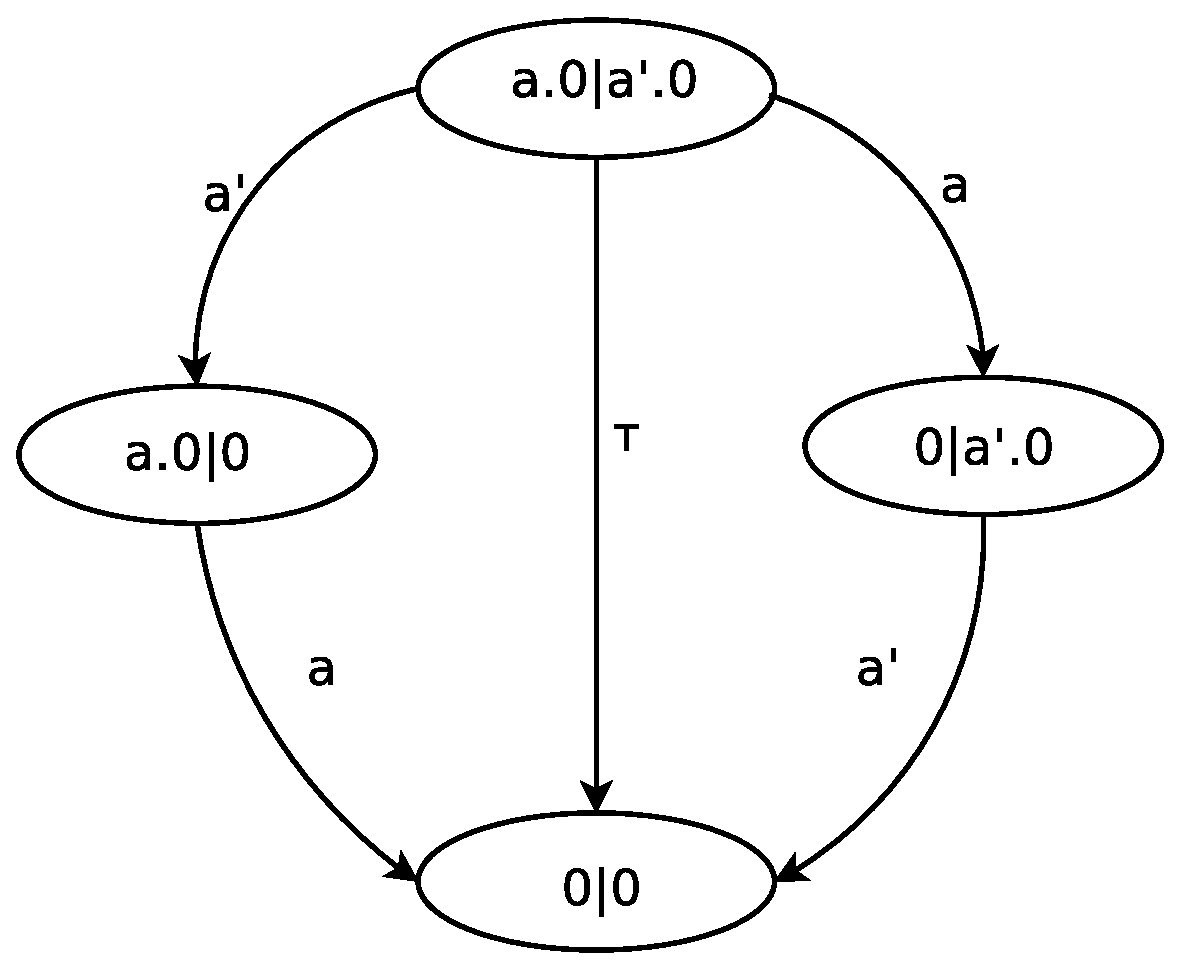
\includegraphics[scale=0.5]{graph1}
  \caption{$\mathit{a.0|\overline{a}.0}$}
  \label{fig:graph1}
\end{figure}

This is illustrated in Fig. \ref{fig:graph1}, where a' represents
$\overline{a}$ and T $\tau$.  To make the derivation of $E|F$
deterministic, the scope of $a$ can be restricted.  In CCS, an input
or output can be paired with any corresponding action which is within
the scope of the channel.  To force the input of $E$ to be paired with
the output of $F$, the scope of $a$ must be restricted so as to only
include the two processes, $E$ and $F$.  This is handled by another
operator in the core syntax, $\backslash$.  The right operand of this
is the name of a channel whose scope is restricted to that of the left
operand.  In this case, $(E|F)\backslash a$ appropriately limits the
possible derivations to just $\derives{\tau}$.

The remaining binary operator within CCS is $+$, which provides
non-deterministic choice between two processes.  Once a derivation is
made from one process, the option of performing the actions of the other
is lost.  This contrasts with the parallel composition operator, where
the other process remains running in parallel.  Choice thus effectively
corresponds to the familiar idea of branching found in sequential
models.  Using the same two exemplar processes again, $E + F$ may derive as
follows:

\begin{enumerate}
\item $E\ +\ F \derives{a} 0$
\item $E\ +\ F \derives{\overline{a}} 0$
\end{enumerate}

\begin{figure}  
  \centering
  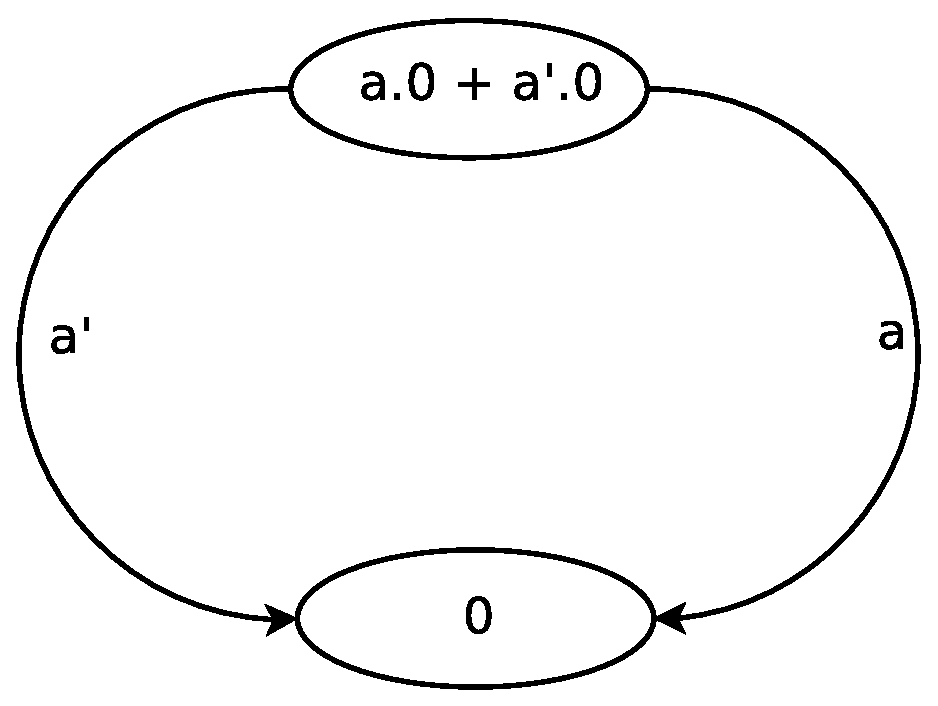
\includegraphics[scale=0.5]{graph2}
  \caption{$\mathit{a.0\ +\ \overline{a}.0}$}
  \label{fig:graph2}
\end{figure}

Again, this is illustrated in Fig. \ref{fig:graph2}.  There are clearly
similarities between the two sets of possible derivations, but note
that, with choice, the option of then executing the remaining process is
lost and there is no possibility of synchronization.

The remaining operators in CCS handle recursion and relabelling.  $\mu
X.E$ binds X with the value of $E$, so that later occurrences of $X$ are
replaced with $E$.  The function, $f$, in $E[f]$ has the type $Act
\rightarrow Act$ and converts actions, while preserving $\tau$ and
complementation.

\subsection{The Dining Philosophers in CCS}

To fully appreciate CCS, it is necessary to see how it may be used to
model a scenario.  Consider the dining philosopher's example
illustrated above. Modelling this in CCS involves first ascertaining
what processes form the basis of this `system'.  Clearly, each
philosopher plays a part, so they should be represented by a process.
Returning to the original definition of the problem, each philosopher
may choose to eat or think.  In CCS, this can be represented as:

\begin{equation}
Philosopher = \mu X.(EatingPhilosopher.X\ +\ ThinkingPhilosopher.X)
\end{equation}

\noindent where the philosopher is recursively defined as making the
choice between becoming an $EatingPhilosopher$ process or a
$ThinkingPhilosopher$ process.  Defining the latter is simple; 
thinking is simply some internal process of the philsopher:

\begin{equation}
ThinkingPhilosopher = \tau
\end{equation}

The focus of the problem is on the eating process, which requires
access to the system's shared resource: the forks.  Modelling this
necessitates defining a protocol whereby the philosopher may interact
with the resource in order to obtain access to it.  From this, it
follows that the forks must also be represented as processes:

\begin{equation}
Fork = \mu X.takeFork.putDownFork.X
\end{equation}

\noindent with two communication channels, $takeFork$ and
$putDownFork$.  The fork begins its life on the table from which it
may be taken, represented here by the reciept of an input on the
$takeFork$ channel.  Once this has occurred, the process becomes
$Fork^\prime$,

\begin{equation}
Fork^\prime = putDownFork.X
\end{equation}

\noindent which represents the state where the fork is in use by a
philosopher.  The fork can't be used again until it has received an
input on $putDownFork$, which causes $X$ to be expanded and the fork to
wait for input on $takeFork$ again.

This interaction is further clarified by defining the final process,
the $EatingPhilosopher$:

\begin{equation}
EatingPhilosopher = \overline{takeFork}.\overline{takeFork}.\tau.\overline{putDownFork}.\overline{putDownFork}
\end{equation}

\noindent which needs to synchronize with two available $Fork$
processes to be able to eat (represented by $\tau$) and then release
the forks.  The system as a whole is modelled by running a number of
philosophers and forks in parallel, and restricting the scope of the
fork channels in order to enforce synchronization.

[Include diagrammatic of this here, showing the processes and channels]

Note that this CCS representation of the problem only models what the
narrative version of the problem above.  There is no attempt to
resolve any of the competition problems, and a strong element of
non-determinism, as to which philosopher gets which fork, still
exists.  It does, however, give a formal representation of the problem
and allows the effects of varying the relative numbers of philosophers
and forks to be observed via execution of the model.

Modifying this slightly allows a model to be obtained that corresponds
exactly to a specified number of philosophers and forks, $n$.  From
the definitions above, multiple variants may be generated, such that
each philosopher and fork process has a unique subscript.  For
example, $Philosopher$ becomes $Philosopher_i$, where $i = 1\dots n$.
The same subscripting also applies to the $takeFork$ and $putDownFork$
channels, so that they now correspond to a specific fork.  The
original solution can thus be represented, as the case where each
philosopher, $i$, initially performs the action $takeFork_i$ (to take
the left fork) and then $takeFork_{i-1}$ (with the exception that when
$i-1 = 0$, we use $n$) \footnote{Again, it is necessary to reverse the
  actions of $Philosopher_n$ in order to obtain a solution that does not
  deadlock}.

This model restricts which fork is taken by which philosopher
(limiting the possible actions, and thus removing some
non-determinism), but is still prone to the effects of
non-deterministic choice (some philosophers may arbitrarily choose to
think instead) and fairness, with regards to action performance (if
the actions are performed in a depth-first manner, only one
philosopher may end up eating).  These may be regarded as
implementational aspects of the model; all these phenomena could be
represented, but a choice between these is not made at this level of
abstraction.

\subsection{Advantages and Limitations of CCS}
\label{ccslimit}

From its syntax, it is clear that CCS can model sequential behaviour
using sequential composition ($\alpha.E$) and non-deterministic choice
($+$).  This further confirms the intuition noted earlier that
sequential programs are a subset of the larger set of concurrent
programs.  This is further illustrated by the $+$ operator, which
returns a smaller set of possible derivations, from the same initial
pair of processes, when compared with parallel composition ($|$).
These sequential operators can also be used to convert a set of
parallel-composed processes into their equivalent interleavings.

CCS can model both sequential and concurrent programs, while still
maintaining a minimal syntax.  However, the calculus is not
Turing-complete\footnote{A finite axiomatisation can be defined, if
  the simultaneous presence of parallel composition and recursion is
  avoided \cite{milner:ccsaxiom}}; there are limitations as to what
may be expressed.  As discussed earlier, Turing completeness does not
necessarily guarantee the suitability of a model for a particular
task. Likewise, the lack of such completeness doesn't imply that the
model is unsuitable.  As shown above, an appropriate model of the
Dining Philosophers problem may be defined, without Turing
completeness.  The lack of this in CCS is not necessarily a problem.
It may even be an advantage in some cases, where this lack of
expressivity simplifies the formal reasoning over the model.

One fairly obvious limitation, and one that is relevant when
discussing Turing completeness, is that there is no data in the model.
The processes discussed so far don't explicitly communicate anything
when they send or receive signals.  Instead, behaviour arises purely
from synchronization.  It is possible to extend CCS to represent this
by adding the concept of value passing between processes.  A host of
other process calculi have been based on such a variant of CCS, and we
will consider this in more detail as part of section \ref{mobility}.

CCS models are also relatively static; while processes may evolve
(e.g. $a.P$ may become $P$) and the number of processes in the system
may change (e.g. a process may branch using parallel composition), the
communication structure doesn't.  Notably, if a process, $E$ knows
about the channels $x$ and $y$ initially, while $F$ only knows about
$x$ (due to restriction on $y$), this status can not change during the
course of the various transitions inherent in the system.

The effect of restriction is more generally known as \emph{scoping}
and occurs frequently with reference to variables in programming
languages.  CCS doesn't allow dynamic changes to the scoping of
channels.  Instead, scoping is fixed to the static arrangement
provided by the initial system, prior to any transitions.  The
addition of dynamic scoping, often referred to as mobility, is the
major contribution of the $\pi$ calculus, a language based on CCS
covered in \ref{scopemobility}.

To conclude, there is another limitation of CCS which is less to do
with a particular concept being absent from the language, instead
being more related to its central aspect: \textbf{synchronization}.
The problem here lies in the \emph{compositionality}\footnote{The
principle of compositionality states that the meaning of the whole
should be derived from the meaning of the parts together with the rules
used to combine them.  As later composition takes place, the same
semantics should still be usable in order to represent a term.} of
processes.  While the structure of a CCS system remains compositional,
as the result of parallel composition is the behaviour of the composed
processes together with the rules of the $|$ operator, this is not true
of the synchronization of multiple processes.

Consider the idea of broadcasting a signal to an arbitrary number of
processes.  Ideally, a general \emph{broadcast agent} should be
defined which provides this behaviour.  In CCS, there are at least two
possible ways of defining semantics for the agent, but not one that
provides a suitably compositional solution.  Perhaps the most obvious
of these is simply to extend the familiar synchronization of two
processes.  An input and output pair can synchronize, so why not just
create multiple pairs, one for each receiving process?  For example,
transmitting a signal to two processes can be written simply as

\begin{equation}
\mathbf{\overline{a}_1.\overline{a}_2.0}\ |\ a_1.P\ |\ a_2.Q
\end{equation}

\noindent where the process on the left (in bold) forms the semantics
for the broadcast agent and the processes, $P$ and $Q$ are the
continuations of the input processes

This will work, but what happens when the broadcast agent needs to
transmit the signal to three processes?

\begin{equation}
\mathbf{\overline{a}_1.\overline{a}_2.\overline{a}_3.0}\ |\ a_1.P\ |\ a_2.Q\ |\ a_3.R
\end{equation}

\noindent The semantics of the broadcast agent have to change.  Simply
composing the third input will lead to one of the three being ignored
by the original definition of the broadcaster given above.  So, simply
enumerating multiple synchronization pairs is not sufficient to
provide a compositional broadcast agent.

A second solution lies in recursion.  If the problem with the previous
solution lies in the broadcasting agent doing too little (i.e. not
transmitting to all the possible receivers), then, by making it
recurse, it will keep sending the output to whoever will synchronize
with it.  Thus, the example for three inputs above becomes

\begin{equation}
\mu X.\overline{o}.X\ |\ o.P\ |\ o.Q\ |\ o.R
\end{equation}

\noindent which works, and will continue to do so if a further
input process is parallel composed.  

But there is still a problem for much the same reasons as the first
solution.  This works fine on this small scale, but what happens when
this agent is placed in the context of a larger system?  Once the agent
starts its cycle of outputs, it won't stop as there exists
no base case for this recursion\footnote{A base case may be introduced
using non-deterministic choice, but there is no guarantee when this will
be invoked, if ever.}.  An output on $o$ will always be available (within
the scope of any restriction placed on that particular channel) and
the broadcasting process can never do anything else.  The result is a
constantly cycling process, which, in an implementation of this model,
would continue to consume resources.

The true solution to this problem is to enable some form of
\emph{global synchronization}.  This requires a separate entity,
disparate from the processes involved in the communication, which can
be used to co-ordinate the synchronization.  In the next section, a
branch of process calculi are considered that provide just such a facility.

\section{Timed Calculi}
\label{timing}

Initially, the use of the word `timed', within the context of the
calculi considered here, is a bit of a misnomer.  The notion of `time'
is generally associated with concrete real values, in units such as
minutes and seconds.  Real-time process calculi, such as those
described in \cite{tccs, satoh:phd, satoh:distrib, lee:realtime,
  aceto:timing, beaten:timing, brics:lee}, attempt to model this.
Instead, this section focuses on a series of discrete timed calculi
which focus on abstract time and the use of \emph{clocks} for the
primary purpose of global synchronization (as described above).

Hennessy's Temporal Process Language (TPL) \cite{hennessy:tpl} extends
the CCS language discussed above with a single clock, akin to a
hardware clock which emits a signal at an arbitrary point in time.
These signal emissions are controlled by a concept known as
\emph{maximal progress}, which allows each process to make as much
progress as possible before the clock ticks.  Formally, this means
that all silent actions ($\tau$s) are performed before a $\sigma$
action (which represents the clock signal) occurs.

This is of little use unless the actions of the processes can actually
depend on the behaviour of the clock.  The two are related via the
addition of a timeout operator.  This takes the form

\begin{equation}
\timeout{E}{\sigma}{F}
\end{equation}

\noindent where $E$ and $F$ are processes and $\sigma$ is the clock.  In
short, $F$ acts if $E$ \emph{times out} on the clock, $\sigma$.  This is
similar to non-deterministic choice, in that only one of the two
processes will ever act and the behaviour of the other is lost.  Here,
however, the choice is determined by the clock (and thus effectively by
the other processes, as it is their behaviour which controls when the
clock will tick).

With these additions, the problem of defining a suitable compositional
broadcast agent, as mentioned above, can be solved.  Recall the second
solution, which used recursion.  Now, with the addition of an external
entity (the clock) and a way of relating it to the processes involved
(timeouts), a base case may be provided via recognition of the point
when no more synchronizations may occur.  This can be added to the
earlier recursive solution

\begin{equation}
\mu X.\timeout{\overline{o}.X}{\sigma}{0}\ |\ o.P\ |\ o.Q\ |\ o.R
\end{equation}

\noindent by simply adding a timeout which stops the recursion.  This
works because the synchronizations of the input processes with the
output of the broadcast agent generate silent actions and thus invoke
maximal progress.  While there is a choice between a silent action
(due to the broadcasting agent synchronizing with an input) and a
clock tick, the silent action always takes precedence and thus every
possible synchronization occurs.  Once no more synchronizations are
possible, the clock is allowed to tick and the recursion stops.

\subsection{Extending TPL}
\label{tplext}

The extensions to TPL considered here focus on expanding the
scalability of the language.  As demonstrated above, TPL adequately
provides for situations where an arbitrary number of processes must
synchronize.  But what happens when a solution, like the one above, is
integrated into a larger system?  With only one clock, further
problems occur.  The use of the clock in one subsystem may conflict
with its use in another, and there is no clock available to
co-ordinate the subsystems themselves.

The Calculus for Synchrony and Asynchrony (CSA) \cite{csa} extends TPL
with the idea of multiple clocks from its predecessor, PMC\footnote{PMC
also differs from TPL in its use of \emph{insistent} actions; all must
be performed before a clock tick.}\cite{pmc}. However, while having
multiple clocks allows the use of differing patterns of synchronization,
it increases the number of clock ticks present within the system.  With
five clocks, even the nil process has five possible transitions (as
clocks idle over nil).

CSA solves this to a limited extent via localising maximal progress to
a pre-defined scope for each clock.  A more elegant solution is
provided in the Calculus for Synchrony and Encapsulation (CaSE)
\cite{CaSE}, which introduces a clock hiding operator into the syntax.
The effect of this is the introduction of \emph{synchronous
  encapsulation}, as hidden clocks emit $\tau$ actions (as opposed to
ticks) outside the operator's scope.  This can be used, in conjunction
with restriction, to produce a hierarchy of components.  The actions
of these subsystems can be represented purely as silent actions, and,
when combined with the global form of maximal progress introduced by
TPL and retained in CaSE, integrated into the `synchronous cycle'
\cite{CaSE} of clocks at the level above.  CaSE is further discussed
in \ref{case}, where it forms the basis for the calculus of
\emph{Typed Nomadic Time} (TNT).

\subsection{Advantages and Disadvantages of Timed Calculi}
\label{timelimit}

The main advantage of the timed calculi we have discussed here is that
they allow, via the introduction of \emph{global synchronization}, the
construction of systems on a larger scale than those that could be
created purely with CCS.  With CaSE, components can be created which
consist of multiple processes and clocks.  These can then be
successfully integrated together to form new components.

Global synchronization allows the problem of defining a compositional
broadcast agent, cited earlier in \ref{ccslimit}, to be solved, but
these timed calculi still retain the other problems with CCS we
mentioned there.  Neither TPL, PMC, CSA or CaSE explicitly include
data within the model.  This is not necessarily a disadvantage; it is
possible to model data implicitly, via the use of silent actions, and
including data in the model complicates formal reasoning and
equivalence theories.

More importantly, these calculi all still retain a static structure.
The scope of restriction or clock hiding doesn't change as the
processes evolve.  This prevents these calculi from being used to
model mobile systems where these elements do change, although they
are perfectly suited to modelling static dataflow-oriented systems
such as those in \cite{WICSA} and \cite{cashews-sem}.

In contrast, the following section contains a discussion of calculi
which, while lacking the scalability of the timed languages just
illustrated, can model \emph{mobile systems}.

\section{Mobility}
\label{mobility}

Within the field of algebraic process calculi, there are two clear ways
in which the dynamic nature of a system is modelled.  The most
well-known is the form of mobility present within Milner's $\pi$
calculus which allows the scope of a name to change as the system
evolves.  This concept can be thought of in a similar way to the
reference passing that occurs in most programming languages; part of the
program begins with no knowledge of an entity, and later gains knowledge
by obtaining a reference to it.

Models in the $\pi$ calculus are not really mobile in the sense of
something moving from one place to another.  This isn't possible, as
there is no real notion of `place' to begin with.  However, the addition
of this mechanism does allow the modelling of dynamic systems, such as a
mobile phone network \cite{milner:lecture}, and is sufficiently
expressive as to allow it to encode Church's $\lambda$ calculus
\cite{funcproc}.

A more naturalistic form of mobility is found in calculi which allow
entities to \emph{migrate}.  One of the primary exponents of this is
Cardelli and Gordon's ambient calculus \cite{amb}, which groups
composed processes inside \emph{ambients}.  These ambients can be
moved up and down a nested hierarchy of such objects, or destroyed.  The
calculus differs from those previously considered, in that it
lacks communication primitives.  Surprisingly, the base syntax is
sufficient to allow communication to be encoded within them, and
indeed the entire asynchronous form of the $\pi$ calculus can be
represented.

The following two sections consider examples of both types of mobile
calculi in more detail.
 
\subsection{Scope Mobility}
\label{scopemobility}

\subsubsection{The $\pi$ Calculus}

The $\pi$ calculus follows on from Milner's earlier work on CCS
discussed in \ref{ccs}. Essentially, it is a value-passing form of CCS
with a generalisation from values and channels in to simple \emph{pure
  names}.  Thus, channels can be passed between processes, as well as
values, which means that their scope may change during execution.

To make this clearer, consider the syntax of the form of $\pi$ calculus
given in \cite{funcproc}

\begin{equation}
\label{pisyntax}
  E, F\ ::=\ 
  0\ |\ 
  \overline{x}y.E\ |\ 
  x(y).E\ |\ 
  (a)E\ |\ 
  (E\ |\ F)\ |\ 
  !E
\end{equation}
  
\noindent which is a minimal version containing replication as opposed
to recursion, with $a$ a channel name and $x$ and $y$ being defined
below.  Compare this with the syntax given for CCS in Eqn.
\ref{ccssyntax}.  The nil process, $0$, is still present, as is parallel
composition and restriction (although in a new form, $(a)E$).
Non-deterministic choice is present in the original version of the $\pi$
calculus presented in \cite{picalctutorial}, but is removed from the
version given in \cite{funcproc} due to the formulation of semantics
used there.  $!E$ is the syntax for replication, which replaces
recursion in this particular variant of the calculus to give a simpler
theoretical treatment, while still doing much the same job.

The main distinction between the two lies in the remaining element of
the syntax: prefixing.  In CCS, a more general syntax,
$\alpha.E$, where $\alpha \in \mathcal{N} \cup \overline{\mathcal{N}}
\cup \{\tau\}$, is used and includes input, output and silent actions.  In the
syntax given above for the $\pi$ calculus, the input ($x(y)$) and output
($\overline{x}y$) syntax are given separately, and the input prefix is
\emph{binding}\footnote{When an input is received on $x$, $y$ is bound
to the value of that input, which is then substituted for $y$ in the
continuation of that process.}. $x$ and $y$ are both names, where `$x$
[is] the \emph{subject} and $y$ the object' \cite{funcproc}.  

The distinction between the $\pi$ calculus and value-passing forms of
CCS, which also use this form of prefixing, lies in $x$ and $y$ being
drawn from the same set in the $\pi$ calculus.  In contrast,
value-passing forms of CCS keep the two sets distinct, so that the
channel and value names do not intersect.  This change is what
gives $\pi$ calculus its power, as channels can now be used as the
object of an input or output.  Thus,

\begin{equation}
x(y).\overline{y}x
\end{equation}

\noindent becomes perfectly valid.

This also has an effect on restriction.  Recall that, in CCS,
$(a.0|\overline{a}.0)\backslash a$ restricts the scope of $a$ to just
the two processes, $a.0$ and $\overline{a}.0$, making a synchronization
the only possible action which may be performed.  Now consider the
following processes defined using the $\pi$ calculus:

\begin{equation}
(a)(a(x).\overline{x}a.0\;|\;\overline{a}y.0)\;|\;y(z).P
\end{equation}

\noindent where the scope of $a$ is again restricted, this time to the
two processes $a(x).\overline{x}a.0$ and $\overline{a}y.0$.  If these
two processes synchronize, the system evolves to:

\begin{equation}
(a)(\overline{y}a.0\;|\;0)\;|\;y(z).P
\end{equation}

\noindent with $x$ becoming bound to the channel name, $y$.  This shows
how the $\pi$ calculus allows channel names to be passed between
processes, but it is the next transition that is really interesting.
$\overline{y}a.0$ will pass the channel name, $a$, to $y(z).P$, which is
outside the scope of the restriction imposed on $a$.  As a result, the
scope of $a$ is \emph{extruded}:

\begin{equation}
(a)(0\;|\;0\;|\;P\{a/z\})
\end{equation}

\noindent so as to include the process, $P$, in which $a$ is now
substituted for $z$.  Further, one of the structural congruence rules of
the $\pi$ calculus \cite{funcproc}:

\begin{equation}
(x)(P\;|\;Q) \equiv P\;|\;(x)Q\text{ if x not free in P}
\end{equation}

\noindent may be used to perform \emph{scope intrusion}, giving:

\begin{equation}
0\;|\;0\;|\;(a)(P\{a/z\})
\end{equation}

\noindent as the channel $a$ no longer occurs in the other two
processes.  These changes in scope are central to the concept of
mobility within the $\pi$ calculus.  They reflect the dynamic
environment of the processes represented, and give the calculus a
greater expressivity.

\subsubsection{Variants of the $\pi$ Calculus}
\label{pivariants}

Multiple variants of the $\pi$ calculus exist, including various
evolutions of the syntax and semantics.  As noted above, replication
is only introduced in the version of the calculus given in
\cite{funcproc}, which also defines a reduction-based semantics.  The
earlier tutorial papers \cite{picalctutorial} instead use recursion
and a structured operational semantics, based on a labelled transition
system.

The polyadic $\pi$ calculus \cite{milner:93polyadic} is a more
distinct variant.  Essentially, this involves a syntactic change to
input and output, so that a tuple is used, as opposed to the single
names used in the monadic $\pi$ calculus\footnote{This is a term used
  to refer to the original $\pi$ calculus in retrospect.}.  Having
this as a core part of the syntax provides advantages in representing
abstractions and giving a natural sort discipline\footnote{Sorts are a
  way of applying typing to the $\pi$ calculus, which will be covered
  further in section \ref{typedcalculi} on typed calculi.}.  However,
it is also possible to simply provide an encoding of this in the
monadic variant.

Doing so is not simply a matter of transmitting each value in
sequence; the operation needs to respect the atomicity implicit in the
use of multiple names.  Observe the following example from
\cite{milner:93polyadic}:

\begin{equation}
x(yz)\;|\;\overline{x}y_1z_1\;|\;\overline{x}y_2z_2
\end{equation}

\noindent wherethe process on the left should receive either $y_1$ and
$z_1$ or $y_2$ and $z_2$.  With the following semantics,

\begin{align}
\seml x(yz) \semr & \eqdef x(y).x(z) \\
\seml \overline{x}yz \semr & \eqdef \overline{x}y.\overline{x}z
\end{align}

\noindent the two sending processes can interfere with one another.
$y$ will become bound to either $y_1$ or $y_2$ on the first
synchronization, which is fine, but $z$ may then receive whichever of
these two remains instead of the second element in the tuple.  This
happens because there is no link between the two synchronizations.
Thus, each subsequent transmission results in a new competition
between the two processes as to who actually synchronizes with the
receiver.

The solution to this problem is to make use of a \emph{private
  channel}.  Before transmitting any of the names that form part of
tuple, the sending process passes a reference to a new channel to the
receiver.  The receiver then uses this channel to receive the contents
of the tuple, rather than relying on an existing channel, which may be
prone to interference.  Thus, the semantics become:

\begin{align}
\seml x(yz) \semr & \eqdef x(w).w(y).w(z) \\
\seml \overline{x}yz \semr & \eqdef (w)(\overline{x}w.\overline{w}y.\overline{w}z)
\end{align}

\noindent where $w$ is the new private channel created to facilitate
the process of transmitting the tuple.  This ability to encode the
polyadic variant in the original monadic calculus implies that the new
syntax fails to yield any greater expressivity, but this is not really
the motivation behind this extension.  Instead, what this provides is
a more natural way of transmitting information, which makes modelling
relatively complex systems easier.

The asynchronous $\pi$ calculus \cite{boudol:asynchrony,
  honda:asynchronouscommunication, sangiorgi:asynchronousprocesscalculi}
  deliberately reduces the level of expressivity in order to simplify
  reasoning and provide a better framework for distributed
  implementations.  The output prefix, $\overline{x}y.E$ is replaced
  with $\overline{x}y.0$, so that there is no continuation after an
  output.  In the original synchronous $\pi$ calculus, the behaviour of
  the continuation, $E$, is blocked until a synchronization with a
  recipient can occur.  This doesn't occur in the asynchronous variant,
  as there is no longer any behaviour dependent on this output
  occurring.

Synchrony can be emulated in the asynchronous polyadic $\pi$ calculus,
just as synchronous messaging frameworks, such as TCP, can be
implemented on top of an asynchronous network.  The receiver simply
has to acknowledge receipt of the message by replying to the sender.
The following semantics are given for the prefixes in \cite{boxedamb01}:

\begin{align}
\seml \overline{c}x.P \semr & \eqdef (r)(\overline{c}xr\;|\;r.P) \\
\seml cy.P \semr & \eqdef c(yr).(\overline{r}\;|\;P)
\end{align}

\noindent where $r$ is not free in $P$.  The output is encoded as the
transmission of a tuple containing two names: $x$, the original name
being sent, and $r$, a new channel created to receive the
acknowledgement from the receipient.  This runs in parallel with
another process that awaits an input on $r$\footnote{$r$ is a
  syntactic abbreviation for $r()$ i.e. the input is an empty tuple.}
before continuing with $P$.  Thus, the original synchronous behaviour
is emulated, as $P$ will not evolve until the receiver has obtained
the private channel, $r$, and replied.

Other changes to the calculus are also commonly adopted to reduce its
expressivity, thus making more proofs feasible.  These include:

\begin{itemize}
\item \emph{input localisation} \cite{merro:locality}, whereby a link
  recieved from another process can not be used for input.  For
  example, a process $a(x).P$ may not use $x$ as a channel upon which
  to receive input in $P$.
\item \emph{uniform receptiveness}
  \cite{sangiorgi:uniformreceptiveness}, where the input end of a link
  occurs only once and is replicated so as to be always available.
\item \emph{input-guarded replication}, which is not just restricted
  to uniform receptiveness variants, but is generally used as a more
  restricted form of replication (so the replication operator becomes
  $!a(x).P$ rather than $!P$).
\end{itemize}

The final variant of the $\pi$ calculus considered here is the
extension to higher-order operations.  The most obvious change to make
in this direction is to allow processes to be exchanged.  Such a
second-order form of the calculus is given by the \emph{Calculus of
  Higher Order Communicating Systems} (CHOCS) \cite{thomsen:chocs},
which actually predates the $\pi$ calculus itself.  This extended CCS
with mobility by allowing processes, rather than channel names, to be
transmitted.

The more general area of higher-order $\pi$ calculus, and the theory
behind it, is covered in Sangiorgi's thesis \cite{sangiorgi:phd}.  It
defines an extension to the $\pi$ calculus, HO$\pi$, which not only
allows the transmission of names (first-order) and processes
(second-order), but also parameterised processes of arbitrarily high
order ($\omega$-order).  This is best illustrated by some examples,
drawn from \cite{sangiorgi:phd}.  In the simplest case, an `executor'
process can be defined, $x(X).X$, which will receive and then execute an
arbitrary process.  Placing this in an appropriate context,

\begin{equation}
\overline{x}P.Q\;|\;x(X).X
\end{equation}

\noindent the process on the left, $\overline{x}P.Q$, will transmit
the process, $P$, to the executor before continuing as $Q$.  Thus,
following the synchronization of the two processes, this system
evolves to become:

\begin{equation}
Q\;|\;P
\end{equation}

\noindent where the process $P$ having being substituted for $X$.  

A more complex example is given by considering Milner's encoding of
the natural numbers \cite{milner:93polyadic}.  A natural number, $n$,
is encoded as a series of outputs on $y$, the number of which is equal
to $n$ (represented as $\overline{y}^n$), followed by a transmission
on $z$ to indicate zero and thus, the end of the number:

\begin{equation}
\seml n \semr \eqdef (y,z)\overline{y}^n.\overline{z}
\end{equation}

\noindent Using HO$\pi$, the addition of these numbers can be encoded
in a very simple way.  In the $\pi$ calculus, summation is achieved
via an indirect reference to the two numbers, using channel names.  In
HO$\pi$, the parameterised processes or \emph{agents} that represent
the numbers can be used directly in the representation of addition.
Thus, actually adding the two numbers together becomes a simple matter
of running the two concurrently, and linking them via a common
channel.

A $Plus$ agent, which performs the addition of two numbers, can be
defined as follows:

\begin{equation}
Plus \eqdef (X,Y)(y,z)((x)(X\langle y,x\rangle \;|\;x.Y\langle y,z\rangle ))
\end{equation}

\noindent where both $X$ and $Y$ are agents with two parameters,
corresponding to $y$ and $z$ respectively in the definition of $\seml
n \semr$ above.  The operation of this agent is best demonstrated by
example.  Assume $X$ is two and $Y$ is three, represented in HO$\pi$ as:

\begin{align}
X(y,z) & \eqdef \overline{y}.\overline{y}.\overline{z} \\
Y(y,z) & \eqdef \overline{y}.\overline{y}.\overline{y}.\overline{z}
\end{align}

\noindent and retaining the same representation used for $\seml n
\semr$ above.  When $X$ and $Y$ are passed to the $Plus$ agent, $X$ is
instantiated with a new private channel, $x$, in place of $z$ in the
above.  $Y$ is then prefixed with an input on this same channel, so
that the $y$ outputs occurring in $Y$ only execute after those in $X$.
This leads to the following sequence of transitions:

\begin{equation}
  \lderives{y} \lderives{y} \lderives{\tau} \lderives{y} \lderives{y} \lderives{y} \lderives{z}
\end{equation}

\noindent which is close to the sequence that occurs for the HO$\pi$
representation of five:

\begin{equation}
  \lderives{y} \lderives{y} \lderives{y} \lderives{y} \lderives{y} \lderives{z}
\end{equation}

Formally, the two are \emph{weakly bisimilar}.  A \emph{bisimulation} is
a symmetric binary relation between two processes, which exists if each
process can simulate the behaviour of the other.  $R$ is such a relation
iff, for all pairs of processes $(p,q)$ in $R$ and all actions,
$\alpha$\footnote{The bisimulation definition given here is more
applicable to the static systems of CCS.  Although it holds for this
simple example, a more detailed method of bisimulation is required to
handle the dynamic binding that occurs in the $\pi$ calculus and its
derivatives.}:

\begin{enumerate}
\item $P \derives{\alpha} P^\prime \implies \exists Q^\prime\ such\
  that\ Q \derives{\alpha} Q^\prime\ and\ (P^\prime,Q^\prime) \in R$
\item $Q \derives{\alpha} Q^\prime \implies \exists P^\prime\ such\
  that\ P \derives{\alpha} P^\prime\ and\ (P^\prime,Q^\prime) \in R$
\end{enumerate}

For a weak bisimulation, $\tau$ transitions are effectively ignored.
A series of such transitions,
$\derives{\tau}\derives{\tau}\derives{\tau}\dots$ is abbreviated to
$\obsderives{\tau}$ and $\obsderives{\tau} \derives{a}
\obsderives{\tau}$ is deemed equivalent to $\derives{a}$.  As the
additional $\tau$ transition in the $Plus$-based derivation is the
only difference between the two, the two can be deemed equivalent
under the rules of weak bisimulation.

Returning to HO$\pi$, the most interesting point about this calculus
is not that it provides the means to formulate abstractions of the
type just demonstrated, but that, in doing so, it adds no further
expressivity.  Indeed, Sangiorgi, in his thesis \cite{sangiorgi:phd}
demonstrates how a HO$\pi$ calculus can be represented in the $\pi$
calculus.  Thus, just as with the polyadic variant, the benefit of
using HO$\pi$ comes not from increased expressivity, but from the
additional ease it provides in modelling certain scenarios.

\subsubsection{The Join Calculus}

The Join calculus \cite{join} takes the asynchronous $\pi$ calculus as
its basis, and focuses on providing a formalism better suited as the
basis for a distributed implementation.

Take the following example $\pi$ calculus process given in [some results in the jc]:

\begin{equation}
x(y).P\;|\;x(z).Q\;|\;\overline{x}a
\end{equation}

\noindent where two processes are waiting to receive input on $x$.
The problem with implementing this in a distributed setting is that
there is no concept of location with the $\pi$ calculus.  Each of the
two receiving processes or \emph{receptors}\footnote{The join calculus
  uses an analogy with chemistry to describe its behaviour, based on
  the \emph{CHemical Abstract Machine} (CHAM) \cite{cham}.} may be
located at an arbitrary distance from both each other and the
transmitter, $\overline{x}a$.  As a result, a \emph{distributed
  consensus problem} arises as to which of the two receptors will
receive the transmission.

The join calculus provides a solution to this problem by altering the
syntax of the $\pi$ calculus.  The asynchronous variant of the
syntax given in Eqn. \ref{pisyntax} becomes:

\begin{align}
\label{joinsyntax}
  P, Q\ & ::=\ 
  0\ |\ 
  \mathtt{def}\ D\ \mathtt{in}\ P\ |\
  (P\;|\;Q)\ |\ 
  x\langle \tilde{v} \rangle \\
  D, E\ & ::=\
  J \rhd P\ |\
  D \wedge E\ |\ 
  \mathbf{T} \\
  J,J^\prime\ & ::=\ 
  x\langle \tilde{v} \rangle\ |\
  (J\;|\;J^\prime)
\end{align}

\noindent with $\mathbf{T}$ being the empty definition and a clear
focus on linking the receptors in $D$ to the emissions occuring in $P$
(both represented by the same syntax, $x\langle \tilde{v} \rangle$).
The use of this is most clearly demonstrated by example:

\begin{equation}
  \mathtt{def}\ (x\langle y \rangle \rhd P) \wedge (x\langle z \rangle \rhd Q)\ \mathtt{in}\ x \langle a \rangle
\end{equation}

\noindent which has essentially the same behaviour as the $\pi$
calculus example presented earlier.  $x\langle y \rangle \rhd P$
receives an input, $y$, on $x$ and then continues as $P$.  $x\langle y
\rangle$ is said to guard $P$, and multiple such guards may be applied
to a single such process.  Multiple such receptors may be defined via
use of the $\wedge$ operator.

It is impossible to provide an exact equivalent to the earlier series
of $\pi$ calculus processes, as the changes in the join calculus now
prevent such scenarios from being created.  Instead, the equivalent of
this join calculus example in the $\pi$ calculus is:

\begin{equation}
(x)(!(x(y).P\;|\;x(z).Q)\;|\;\overline{x}a)
\end{equation}

\noindent where the scope of $x$ is restricted to the $\mathtt{def}$
expression and the inputs are replicated, so as to be always
available.  Thus, a channel $x$ is always \emph{localized} to a
particular set of emitters and receptors.

Clearly, the join calculus, as a reformulation of the asynchronoous
$\pi$ calculus with a new syntax, can not be used to express anything
which can't be expressed in the $\pi$ calculus.  However, it has a lot
of advantages in endowing the calculus with distributive properties at
the syntactic level\footnote{Such changes have also been made using the
restrictions imposed by an appropriate type system}

\subsubsection{Advantages and Disadvantages of the $\pi$ Calculus}

The $\pi$ calculus is a powerful formalism drawn from a minimal
abstract syntax.  As noted at the start of this section, it is capable
of encoding the $\lambda$ calculus and so it follows that it is also
capable of simulating any recursive function.

The problem is that this makes it a little too powerful in some cases.
From \cite{sangiorgi:types-or}, we can see how much more difficult the
additional power given by the $\pi$ calculus makes proving
termination.  In contrast, a sufficiently restricted form of CCS
provides a trivial proof.  In the same paper, Sangiorgi also touches
on something which seems common within the literature
\cite{join,stefani:kells,wojciechowski:phd,failure2}; while the
expressiveness of the $\pi$ calculus is interesting, it is necessary
to restrict it in order to actually have something which is generally
useful for reasoning over or using as the basis for a full programming
language.  Specifically, to prove termination for the $\pi$ calculus,
it is necessary to employ the asynchronous variant with uniform
receptiveness and the input-guarded replication operator.

Another problem with the $\pi$ calculus is that it carries with it a
trait from CCS.  Namely, it can't be used to model synchronization
with an arbitrary number of processes in a compositional way.  This
was considered earlier in \ref{ccslimit} for CCS, and solved in
\ref{timing} using the additions to the calculus given by TPL.  While
the $\pi$ calculus has a notion of mobility and is thus more
expressive than CCS, it still lacks an external entity with which to
co-ordinate such a transaction.  

A common motif reoccurs here, that was touched on earlier in the
introduction to this review; even though something has a certain level
of expressivity, it doesn't follow that it is the most appropriate
mechanism for modelling a particular phenomenon.  This also holds for
the distributed calculi considered in \ref{migration}.  The $\pi$
calculus may already model mobility, but these calculi do so in a
different way, which may prove more suitable in a particular context.
 
\subsection{Distribution and Migration}
\label{migration}

Allowing the scope of a name to change during execution is one possible
way of modelling dynamic behaviour, but it isn't the only way.  The
concept of \emph{mobility} naively implies the physical movement of
processes, but, as shown above, this is not what actually happens in the
$\pi$ calculus.  To do so requires some notion of \emph{distribution};
this can be provided by \emph{localities}, a term used to refer
generally to a higher-level form of grouping, above that of processes.
This concept has been applied to various calculi, in different forms, in
order to model physical sites \cite{wojciechowski:phd}, administrative
or security domains \cite{amb,seal} and biological cells \cite{brane04},
but can theoretically be applied in any context where the grouping of
processes is useful.  Localities can be used simply for observation or
as a means to further control the behaviour of the processes
encapsulated within them.  They are generally named, so as to provide a
communication target or a known destination for a migrating entity.

Originally, localities were used to distinguish between processes in
order to provide further equivalence theories.  Take the following simple
CCS-based example process:

\begin{equation}
\label{lccsspec}
Spec \eqdef in.\tau.\overline{out}.Spec
\end{equation}

\noindent which forms the \emph{specification} for the behaviour of a
system that receives an input, processes it and then returns the output.
The actual \emph{implementation} may differ from the specification by
instead involving two processes:

\begin{align}
\label{lccs2proc}
Receiver & \eqdef in.\overline{a}.Receiver \\
Sender & \eqdef a.\tau.\overline{out}.Sender
\end{align}

\noindent which communicate over another channel, $a$.  If these two
processes are run concurrently:

\begin{equation}
(Receiver\;|\;Sender)\setminus a
\end{equation}

\noindent with the scope of $a$ restricted, they are \emph{weakly
bisimilar} (see \ref{pivariants}) to one another.  The specification
performs the following derivations:

\begin{equation}
  \lderives{in} \lderives{\tau} \lderives{\overline{out}}
\end{equation}

\noindent prior to recursing and becoming $Spec$ again, whereas the
implementation produces:

\begin{equation}
  \lderives{in} \lderives{\tau} \lderives{\tau} \lderives{\overline{out}}
\end{equation}

\noindent with the extra $\tau$ transition caused by the synchronization
on $a$.  As weak bisimulation effectively ignores $\tau$ actions, the
two are judged to be equivalent.  If the specification was to include a
further $\tau$ action, for an arbitrary reason, prior to the
$\overline{out}$, then the two would also be strongly bisimilar.  To
summarise, the difference between the two sets of derivations is
negligible, according to the equivalence theory, yet the actual
difference between the specification and its implementation is fairly
significant.  The specification effectively requests a monolithic
solution, but weak bisimulation allows the final implementation to be
distributed over multiple processes.

In most situations, this is beneficial.  It means that the specification
can be met by a concurrent system, composed of multiple processes
running in parallel, superfluous $\tau$ transitions aside.  When a
distinction between the number of processes used is required, a finer
equivalence is needed.  \emph{Location bisimulation} \cite{obslocal}
provides exactly that, by assigning locations to processes and using
them as part of the relation between processes.

Essentially, this means that each transition is annotated with a
location name.  A variant of CCS, LCCS, adds an additional piece of
syntax, $l::E$ to signify that a process $E$ is located at $l$.  This
association is made within the operational semantics, of which there are
two variants.  The \emph{static} approach allocates locations initially,
while the \emph{dynamic} method generates a new location for each
non-silent transition.  Here, the focus is on the latter, shown in Table
\ref{tab:lccssemantics}, which essentially gives each process a
\emph{causal path}, by explicitly representing the number of transitions
that have been performed.

\begin{table}
  \caption{LCCS Dynamic SOS Rules}
  \label{tab:lccssemantics}
  \shrule
 \begin{center}
    \begin{tabular}{lcr}
      \Rule{\textsf{Act1}}
      {-}
      {a . E \xrightarrow[l]{a} l::E}
      {for\ any\ l \in Loc}
      &
      \Rule{\textsf{Act2}}{E \xrightarrow[u]{a} E^\prime}
      {l::E \xrightarrow[lu]{a} l::E^\prime}
      {}
      &
      \Rule{\textsf{Act3}}
      {-}
      {\tau . E \derives{\tau} E}
      {}
     \end{tabular}
  \end{center}
 \shrule
\end{table}

The semantics, as with those for CaSE and TNT given in chapter
\ref{currentwork}, are based on a \emph{labelled transition system}.
The possible behaviour of a process is defined as a series of labelled
transitions from one process to another, which are later used as the
basis for the bisimulation-based equivalence theories shown earlier.
The rules presented here are only a subset of those for LCCS, being
those that are relevant to the use of locations.  The remaining rules
for summation, parallel composition and restriction are as for CCS
itself, with the additional inclusion of the location on the transition.
These are discussed informally in section \ref{ccs}, and also appear as
part of the CaSE semantics.  

The rule, $Act1$, handles the initial assignment of a location for any
action, $a.E$, where $a \in \mathcal{N} \cup \overline{\mathcal{N}}$
(i.e. $a \ne \tau$) and $Loc$ is simply a set of location names.  The
rule states that the process may perform a transition to the process
$l::E$.  The transition itself is annotated with both the action $a$ and
the new location, $l$, which causes the locations to appear in the
sequence of transitions for each process (and, thus, the equivalence
theory).

$Act2$ is a continuation of $Act1$, which handles processes that have
already been assigned a location.  If the process itself, $E$, can
perform some action, $a$, with the location, $u$, to become $E^\prime$,
then so can the located version of $E$.  The interesting part of this
rule is how the location is used in the new transition.  The $u$ from
the new transition is concatenated with the $l$ from the current
location, so the transition depicts the specific route the process has
taken through each location.  The final rule, $Act3$, simply handles
silent actions, which are unaltered from their behaviour in CCS, and
have no association with locations.

How this actually works in practice is best shown by reconsidering the
earlier CCS example.  Recall the specification defined in
\ref{lccsspec}.  This is a process with essentially three actions, $in$,
$\tau$ and $\overline{out}$, which may be localised via use of the LCCS
semantics given above.  As the process begins its life in an unlocated
form, $Act1$ is applied to assign it a location:

\begin{equation}
in.\tau.\overline{out}.Spec \locderives{l}{in}
l::\tau.\overline{out}.Spec
\end{equation}

\noindent where $l$ is an arbitrary location name\footnote{The name is
arbitrary in the sense that it doesn't matter what the name is, but, as
the later discussion of bisimulation shows, the location names must be
assigned in some kind of regular fashion to facilitate comparison}.  The
evolution of the resulting process, $l::\tau.\overline{out}.Spec$
utilises both $Act2$ and $Act3$.  $Act2$ provides the appropriate
transition for such a located process, but its behaviour is based on
that of the unlocated process, which in this case is
$\tau.\overline{out}.Spec$.  Thus, $Act3$ is used to yield:

\begin{equation}
\tau.\overline{out}.Spec \derives{\tau} \overline{out}.Spec
\end{equation}

\noindent which is then applied as the precondition for $Act2$ to give:

\begin{equation}
l::\tau.\overline{out}.Spec \locderives{l}{\tau} l::\overline{out}.Spec
\end{equation}

\noindent As $u$ is effectively the empty string, $\epsilon$, in this
case, due to the $\tau$ transition being unlocated, the result of the
concatenation, $ul$, is simply $l$.

The final derivation again combines the use of $Act2$ with another rule.
This time, the action is a member of $\overline{\mathcal{N}}$, so $Act1$
is used to give the derivation of the unlocated variant,
$\overline{out}.Spec$:

\begin{equation}
\overline{out}.Spec \locderives{k}{\overline{out}} k::Spec
\end{equation}

\noindent where $k$ is again an arbitrary location assigned to the new
visible action.  Merging this with the main process using $Act2$ gives:

\begin{equation}
l::\overline{out}.Spec \locderives{lk}{\overline{out}} l::k::Spec
\end{equation}

\noindent resulting in a final process with a causal path of two
locations, $l$ and $k$.

But how does this help distinguish the specification from its dual
process implementation shown previously?  First, it is necessary to
extend the definition of bisimulation given in \ref{pivariants} to
incorporate the localised transitions of LCCS.  Recall that a
\emph{bisimulation} is a symmetric binary relation between two
processes, which exists if each process can simulate the behaviour of
the other.  $R \subseteq LCCS \times LCCS$ is a \emph{dynamic location
bisimulation} relation iff, $\forall (p,q) \in R \wedge a \in \mathcal{N}
\cup \overline{\mathcal{N}} \wedge u \in Loc$:

\begin{enumerate}
\item $P \locderives{u}{a} P^\prime \implies \exists Q^\prime\ such\
  that\ Q \locderives{u}{a} Q^\prime\ and\ (P^\prime,Q^\prime) \in R$
\item $Q \locderives{u}{a} Q^\prime \implies \exists P^\prime\ such\
  that\ P \locderives{u}{a} P^\prime\ and\ (P^\prime,Q^\prime) \in R$
\item $P \derives{\tau} P^\prime \implies \exists Q^\prime\ such\
  that\ Q \derives{\tau} Q^\prime\ and\ (P^\prime,Q^\prime) \in R$
\item $Q \derives{\tau} Q^\prime \implies \exists P^\prime\ such\
  that\ P \derives{\tau} P^\prime\ and\ (P^\prime,Q^\prime) \in R$
\end{enumerate}

\noindent This is the strong variant that observes $\tau$ transitions.
A localised version of weak bisimulation merely requires satisfying the
first two conditions.  As the earlier comparison between the two
processes was made using weak bisimulation, it is this weak variant of
dynamic location bisimulation that will be used here.

The implementation with two processes, shown in \ref{lccs2proc}, had the
following transitions using plain CCS:

\begin{equation}
  \lderives{in} \lderives{\tau} \lderives{\tau} \lderives{\overline{out}}
\end{equation}

\noindent whereas the specification exhibits the following behaviour in
LCCS:

\begin{equation}
  \locderives{l}{in} \locderives{l}{\tau} \locderives{l}{\tau} \locderives{lk}{\overline{out}}
\end{equation}

\noindent To compare the two, it is necessary to give a similar
localised treatment to the transitions for the implementation.  Clearly,
the $\tau$ transitions will be relatively unaffected, and, under a weak
form of bisimulation, are irrelevant anyway.  Essentially, the two
sequences being compared are:

\begin{align}
& \locderives{l}{in} \locderives{lk}{\overline{out}} \tag{Specification
(Localised)} \\
& \lderives{in} \lderives{\overline{out}} \tag{Implementation}
\end{align}

\noindent when the $\tau$ transitions are ignored.  To localise the
latter of these, it is necessary to look back to the original two
processes from which these transitions are derived.  The first,
$\lderives{in}$, arises from the $Receiver$ as follows:

\begin{equation}
in.\overline{a}.Reciever \derives{in} \overline{a}.Reciever
\end{equation}

\noindent which, when localised, becomes:

\begin{equation}
in.\overline{a}.Receiver \locderives{l}{in} l::\overline{a}.Reciever
\end{equation}

\noindent So, the first of the two transitions should be
$\locderives{l}{in}$ when LCCS is used.

However, the use of $a$ makes things a little complicated.  It appears
in both the $Receiver$ (as just shown) and the $Sender$ as a visible
action ($a$ and $\overline{a}$ respectively), but these combine to
become a $\tau$ action when the two are run in parallel.  The above
makes it appear that the $Receiver$ will evolve to $l::k::Receiver$, by
assigning a further location to $a$, but this doesn't match with the
higher-level behaviour of the composed processes.  Thus, to make
assigning locations easier, it is better to look instead at the
sequences of transitions from each process, rather than their explicit
definitions:

\begin{align}
& \lderives{in} \lderives{\tau} \tag{Receiver} \\
& \lderives{\tau} \lderives{\tau} \lderives{\overline{out}} \tag{Sender}
\end{align}

\noindent where the $\tau$ transition arising from the synchronization
is given for both.  From this, it is a simple matter of assigning a
location to each observable action:

\begin{align}
& \locderives{l}{in} \lderives{\tau} \tag{Localised Receiver} \\
& \lderives{\tau} \lderives{\tau} \locderives{l}{\overline{out}}
\tag{Localised Sender}
\end{align}

and merging the two to give a localised version of both the
specification and its implementation:

\begin{align}
& \locderives{l}{in} \locderives{lk}{\overline{out}} \tag{Specification
(Localised)} \\
& \locderives{l}{in} \locderives{l}{\overline{out}} \tag{Implementation (Localised)}
\end{align}

\noindent which illustrates a clear difference between the two.

For the first transition, the two can match each other, as both are
capable of performing $\locderives{l}{in}$.  However, the relation
breaks down on the second transition which compares $\locderives{lk}{\overline{out}}$
with $\locderives{l}{\overline{out}}$.  Under a normal weak
bisimulation, these two transitions would be judged equivalent, as only
the action is available for comparison; both perform an
$\overline{out}$.  However, a localised bisimulation requires the
locations to also match, which fails here.  The specification has a
longer causal path, as its single process has performed two visible
actions.  In contrast, the two processes involved in the implementation
have performed one action each, resulting in two separate paths with a
length of one.

This shows that localities can be used to provide a stronger equivalence
theory; a dynamic location bisimulation can distinguish more processes
than a standard bisimulation.  As stated earlier, localities are now
more commonly used in calculi which exhibit mobility in the form of
\emph{migration}, where they are used to group arbitrary numbers of
processes.  The locality gives the grouping a context, which may change
during execution of the system, via the movement of the locality or its
constituent processes.  What follows is a further examination of such
distributed calculi, including those which have arisen from existing
non-distributed formalisms, such as the $\pi$ calculus.

\subsubsection{The Distributed $\pi$ Calculus}

The distributed $\pi$ calculus, or D$\pi$ \cite{hennessy:dpi98},

\subsubsection{The Distributed Join Calculus}

\cite{djoin} defines a distributed variant of the Join calculus

\subsubsection{Nomadic Pict}

Pawel Wojciechowski defines, in his PhD thesis \cite{wojciechowski:phd},
an extension to PICT \cite{daveturner:phd} which incorporates
distribution.

\subsubsection{The Ambient Calculus}
\label{ambientcalculus}

The ambients within the ambient calculus \cite{amb} are a form of
locality.  Each ambient can contain processes and other ambients,
allowing a nested structure of ambients to be formed.  This topology
is dynamic; new ambients may be created and existing ones moved or
destroyed during execution.  Within the formal syntax of the calculus,

\begin{equation}
\label{ambsyntax}
  E, F\ ::=\ 
  0\ |\ 
  M.E\ |\ 
  (\nu n)E\ |\ 
  (E\ |\ F)\ |\ 
  n[E]\ |\ 
  !E
\end{equation}

\noindent the ambients are represented by the term $n[E]$, where $n$
is an ambient name.  In comparing this with the syntax given for CCS
in Eqn. \ref{ccssyntax} and that of the $\pi$ calculus from Eqn.
\ref{pisyntax}, some apparent similarities can be seen, especially
with regard to the latter.  The same nil process, $0$, is present, as
is parallel composition and replication.  $(\nu n)E$ looks similar to
restriction\footnote{This is the syntax used in versions of the $\pi$
  calculus later than \cite{funcproc}.}.  Continuing on this
presumption, $M.E$ may be considered to be the prefixing already seen
in CCS and the $\pi$ calculus.  However, the syntax for $M$ is

\begin{equation}
\label{ambsyntaxcap}
  M\ ::=\ 
  in\ n\ |\
  out\ n\ | \
  open\ n
\end{equation}

\noindent which is quite different from that of action prefixing.  The
ambient calculus has no concept of channels; the only names present
refer to ambients (so $(\nu n)E$ restricts these).  What $M$ provides
is a set of mobility primitives, known as \emph{capabilities}.
Processes emit these in order to alter the structuring of the
ambients, and thus perform the physical migration of ambients and the
processes within them.

Perhaps the most confusing aspect of capabilities is that they are
emitted by the process, but it is the ambient that actually moves.
For example, if process $P$ is defined as $in\ n.0$, then performing
this action has the effect of moving the \emph{ambient} in which $P$
resides inside $n$, rather than just $P$.  Likewise, $out\ n$ is the
converse and moves the surrounding ambient outside $n$.

Such behaviour is best illustrated by an example. The process, $in\
n.out\ n.P$ begins its life in the ambient $m$
(Fig. \ref{fig:ambient1}).  Performing the first action, $in\ n$,
moves its surrounding ambient, $m$, inside $n$
(Fig. \ref{fig:ambient2}).  The converse, $out\ n$, then moves $m$
back outside $n$, resulting in a return to the original ambient
structure (Fig. \ref{fig:ambient3}), but with the process having
evolved in to $P$.

\begin{figure}  
  \centering
  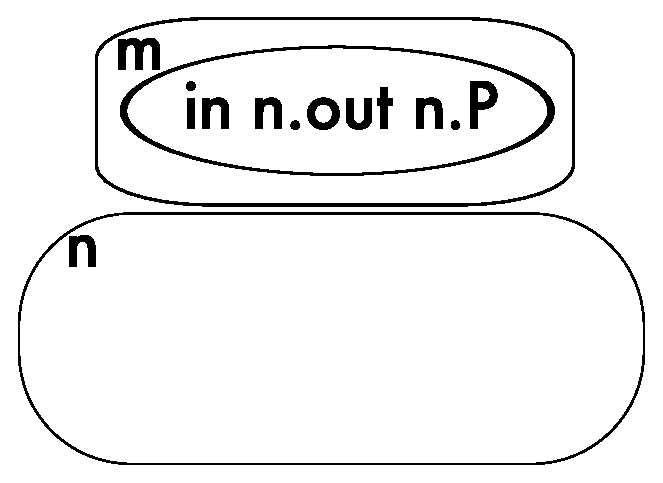
\includegraphics{ambient1}
  \caption{\textit{in n.out n.P}}
  \label{fig:ambient1}
\end{figure}

\begin{figure}  
  \centering
  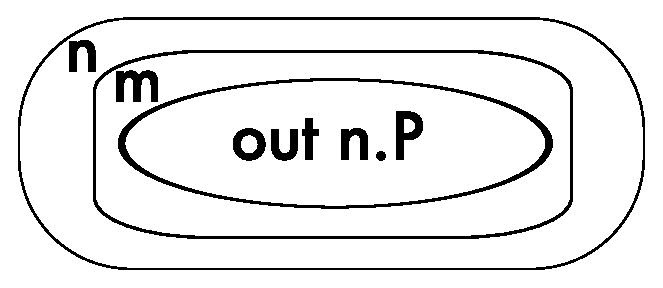
\includegraphics{ambient2}
  \caption{\textit{out n.P}}
  \label{fig:ambient2}
\end{figure}

\begin{figure}  
  \centering
  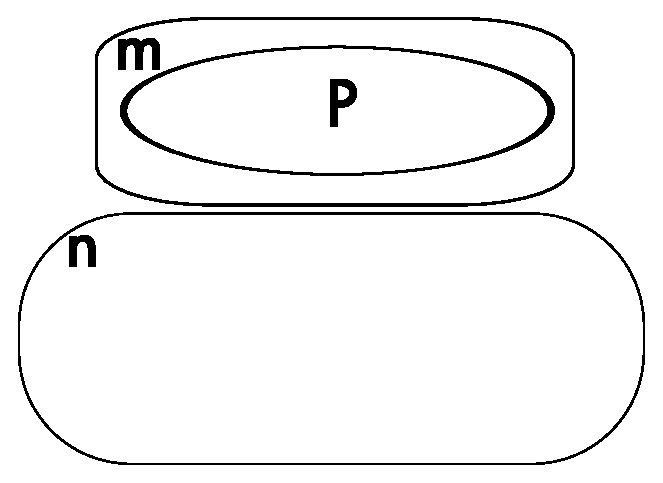
\includegraphics{ambient3}
  \caption{\textit{P}}
  \label{fig:ambient3}
\end{figure}

$open\ n$ is quite different.  It alters the structure, just as $in$ and
$out$ do, but rather than moving ambients, it destroys them.  It is also
applied to a child ambient rather than to the surrounding ambient, so
$open\ m.P\ |\ m[Q]$ (as in \cite{amb}) reduces to $P\ |\ Q$.

There are also issues with regard to the applicability of capabilities
and the use of the names.  A capability may only cause movement to occur
when at least one applicable ambient is available.  As such, movement
is heavily dependent on context, and specifically the availability of an
appropriately named ambient.  Applicability is dependent upon the
capability involved:

\begin{itemize}
\item For $\ambin{m}$, there must be a sibling of the surrounding
ambient named $m$.
\item For $\ambout{m}$, the parent of the surrounding ambient must be
named $m$.
\item For $\ambopen{m}$, there must be a sibling ambient named $m$.
\end{itemize}

All three capabilities are non-deterministic.  The same ambient name may
occur more than once, and each occurrence is regarded as being distinct.
As a result, the reduction of a capability includes a choice if there is
more than one applicable ambient present.  For example, $open\ m.P\ |\
m[Q]\ |\ m[R]$ has two possible derivations,

\begin{enumerate}
\item $open\ m.P\ |\ m[Q]\ |\ m[R] \rightarrow P\ |\ Q\ |\ m[R]$
\item $open\ m.P\ |\ m[Q]\ |\ m[R] \rightarrow P\ |\ m[Q]\ |\ R$
\end{enumerate}

The issue of non-determinism illustrates the behaviour that occurs when
there is more than one applicable ambient.  What about when there are
none?  The process stalls, and can not move on until such an ambient
becomes available.  This is akin to the situation in channel-based
calculi, such as CCS or the $\pi$ calculus, where a name is restricted,
but the appropriate co-name is not available to provide synchronization.
For example,

\begin{equation}
(a.P) \backslash a 
\end{equation}

\noindent may never progress to become $P$ as there is no $\overline{a}$
for $a$ to synchronize with.  This behaviour is particularly relevant
with respect to $\ambout{m}$, where the sole use of the name is to stop
the surrounding ambient leaving its parent if the names don't match.

The restriction of ambient names, via $(\nu n) \expr$, combined with
mobility means that scope extrusion is also present in the calculus.
Just as the transmission of a name outside its scope causes extrusion
in the $\pi$ calculus, the restriction of ambient names may float
outward as necessary.  Scope intrusion is also possible in both
calculi, as demonstrated by the presence of the structural congruence
rule,

\begin{equation}
(\nu n)(P \pc Q) \equiv P \pc (\nu n) Q\ if\ n \not \in fn(P) \tag{Struct Res Par}
\end{equation}

\noindent which allows the restriction of $n$ to be removed from $P$
if the name doesn't occur free within its body.

\subsubsection{Variants of the Ambient Calculus}
\label{ambvariants}

A general problem within concurrency is the possibility of
\emph{interference}.  This was touched on briefly in the introduction
to this review, where the value of $x$ differed due to a race
condition.  In the ambient calculus, \emph{redex interference}
\cite{sangiorgi:mobsafeambients} is an issue, and is related to the
non-determinism mentioned above.

Take the example process from \cite{sangiorgi:mobsafeambients}.

\begin{equation}
n[\ambin{m}.P] \pc m[Q] \pc m[R]
\end{equation}

\noindent It is unclear what the environment of $P$ will be, following
the reduction of the capability, $\ambin{m}$.  There are two
alternatives,

\begin{enumerate}
\item $n[\ambin{m}.P] \pc m[Q] \pc m[R] \rightarrow m[n[P] \pc Q] \pc m[R]$
\item $n[\ambin{m}.P] \pc m[Q] \pc m[R] \rightarrow m[Q] \pc m[n[P] \pc [R]]$
\end{enumerate}

\noindent resulting from the two redexs formed between
$n[\ambin{m}.P]$ and $m[Q]$, and $n[\ambin{m}.P]$ and $m[R]$.  If one
contracts, resulting in a reduction, the other is no longer possible.
However, in this case, at least all three processes, $P$, $Q$ and $R$,
can still interact following either reduction.

In another example from the same paper,

\begin{equation}
\ambopen{n}.P \pc \ambopen{n}.Q \pc n[R]
\end{equation}

\noindent again with two possible interactions

\begin{enumerate}
\item $\ambopen{n}.P \pc \ambopen{n}.Q \pc n[R] \rightarrow P \pc open
  n.Q \pc R$
\item $\ambopen{n}.P \pc \ambopen{n}.Q \pc n[R] \rightarrow
  \ambopen{n}.P \pc Q \pc R$
\end{enumerate}


\noindent the resulting process includes a process, either $open n.Q$
or $open n.P$, which is stuck until such a time as another ambient
named $n$ appears as a parent.  This may never occur.  These kind of
interferences, referred to in \cite{sangiorgi:mobsafeambients} as
\emph{plain interferences}, may occur in other calculi.  The equivalent
in the $\pi$ calculus would be:

\begin{equation}
\overline{x}z.P \pc x(y).Q \pc x(y).R
\end{equation}

\noindent where again a reduction will occur between one of the two:

\begin{enumerate}
\item $\overline{x}z.P \pc x(y).Q \pc x(y).R \rightarrow P \pc Q\{z/y\}
  \pc x(y).R$
\item $\overline{x}z.P \pc x(y).Q \pc x(y).R \rightarrow P \pc x(y).Q
  \pc R\{z/y\}$
\end{enumerate}

\noindent and the remaining process, either $x(y).Q$ or $x(y).R$, will
be blocked.

Another more serious form of interference may occur in the ambient
calculus, due to the provision of differing interactions ($\ambin{m},
\ambout{m} and \ambopen{m}$).  These \emph{grave interferences} occur
when an ambient is involved in two reductions occurring as the result
of different types of capability.  Take the example process,

\begin{equation}
\ambopen{n}.\nil \pc n[\ambin{m}.P] \pc m[Q]
\end{equation}

\noindent in which two reductions can occur that are logically
different.  While the interferences described above are a
representation of the kind of race conditions and non-determinism that
would be expected in any concurrent model, for example, to represent
competition for resources, grave interferences are usually unexpected.
This process may perform two radically different reductions,

\begin{enumerate}
\item $\ambopen{n}.\nil \pc n[\ambin{m}.P] \pc m[Q] \rightarrow \nil \pc \ambin{m}.P \pc m[Q]$
\item $\ambopen{n}.\nil \pc n[\ambin{m}.P] \pc m[Q] \rightarrow \ambopen{n}.\nil \pc m[n[P] \pc Q]$
\end{enumerate}

\noindent where either $n$ is destroyed, thus preventing the latter
movement of $P$ in to $m$ as it has no surrounding ambient, or $n$
moves inside $m$ and is no longer available to be destroyed by
$\ambopen{n}.\nil$.

\subsubsection{Advantages and Disadvantages of the Ambient Calculus}

The most interesting aspect of the ambient calculus is that, while it
includes no communication primitives, it can encode the asynchronous
$\pi$ calculus (see \ref{pivariants}).  This seems to imply that it is
possible to model mobility in a more natural way without losing much of
the expressivity of the $\pi$ calculus.  This seems a little less
surprising when we consider that ambient names exhibit the same scope
extrusion we see with channel names in the $\pi$ calculus.  With this in
mind, it is not too difficult to see that ambient names could be used to
mimic channel names, with synchronization being emulated by two
processes performing some kind of interaction within the same ambient.

However, the representation of synchronization illustrated in \cite{amb}
seems to suggest that the ambient calculus may still have problems
dealing with the kind of global synchronization needed for the broadcast
agent we considered earlier in \ref{ccslimit}.  The operation is
performed by destroying and recreating ambients, as a signal to the
other process involved in the synchronization.  Extending this would
seem to require using more ambients, which again leads us into the
problem of enumerating the number of entities who wish to synchronize.
As we saw before, this is possible but not compositional; every time we
need to perform the synchronization with a different number of agents,
we need to recreate the semantics for the process.

Thus, the ambient calculus and the $\pi$ calculus have more in common
than is initially apparent, and the choice between the two seems to be
largely based on whichever is most natural for a particular task.

\subsubsection{The Seal Calculus}

The seal calculus \cite{seal}

\subsubsection{P Systems}
\label{psystems}

\subsubsection{Bigraphs}
\label{bigraphs}

\section{Typed Calculi}
\label{typedcalculi}

\subsection{Type Systems for the $\pi$ Calculus}

\subsubsection{Sorts}
\subsubsection{Typing for Termination}
\subsubsection{The Type System of the Distributed $\pi$ Calculus}

\subsection{Type Systems for the Ambient Calculus}
\label{ambienttypes}

\subsubsection{Groups}
\label{ambientgroups}

\subsubsection{Single Threadedness}

\section{Biological Applications}
\label{bioapps}

\subsection{The Stochastic $\pi$ Calculus}

\subsection{Bioambients}

\subsection{Quorum Sensing}
\label{quorumsensing}

\section{Conclusion}

\textbf{TODO: Extend to represent added sections}

To conclude, we have taken a brief look at the field of concurrency from
the perspective of algebraic process calculi.  Initially, we saw that,
while universal Turing machines and the $\lambda$ calculus can simulate
any recursive function, their inherent sequential behaviour makes them
unsuitable for modelling concurrent systems.  CCS, in contrast, is less
expressive but can model this kind of behaviour.

The $\pi$ calculus seems to provide the best of both worlds, being able
to model concurrent systems and still retain the expressiveness of the
$\lambda$ calculus.  However, we identified a key limitation which
reasserted our original claim that expressivity only makes a model
capable, and not suitable, for simulating any recursive function;
modelling global synchronization via a broadcasting agent.  This
limitation seems to hold for both CCS and the $\pi$ calculus, and it is
also likely that it applies to the ambient calculus, a formalism that
provides a more natural form of mobility via structural changes.

However, the series of timed calculi that we considered overcame this.
We were able to use TPL to model a broadcasting agent using semantics
suitable for any arbitrary number of processes.  We also saw how
extensions to the language, such as CaSE, could scale even further using
synchronous encapsulation to create systems of multiple components.

What seems to be lacking is a calculus which combines both the mobility
we've seen in the $\pi$ and ambient calculi with the inherent
scalability of a calculus like CaSE.  This is what we hope our research
will be able to provide.




\chapter{Current Work}
\label{currentwork}

The aim of this research is to construct a process calculus which
combines the notions of discrete time and mobility.  Earlier work
during an undergraduate project focused on developing a semantics for
the Cashews\footnote{Cashews is a language for web service
  composition, initially based on OWL-S.}\cite{cashews-sem} language,
using the CaSE process calculus (see section \ref{tplext}) and later,
a conservative extension to it called Cashew-Nuts.  It became clear
during this project that it would be interesting to further extend CaSE
with a notion of mobility, and this lead to the development of the
calculus of \emph{Typed Nomadic Time} (TNT) discussed here.

\section{The Calculus of Synchronous \\ Encapsulation (CaSE)}
\label{case}

The syntax for CaSE, given in \cite{norton05alg}, is as follows:

\begin{equation}
  \begin{aligned}
    \expr, \exprb\ ::=\ &
    \nil  \;\,|\,\; 
    \Delta \;\,|\,\; 
    \Delta_{\sigma} \;\,|\,\; 
    \alpha . \expr  \;\,|\,\;
    \expr + \exprb \;\,|\,\; 
    (\expr\;|\;\exprb)\;\,|\,\; 
    \timeout{\expr}{\sigma}{\exprb} \;\,|\,\; \\
    & \stimeout{\expr}{\sigma}{\exprb} \;\,|\,\; 
    \mu X . \expr \;\,|\,\; 
    X \;\,|\,\; 
    \expr \setminus a \;\,|\,\; 
    \expr / \sigma
  \end{aligned}
\end{equation}

\noindent where $\alpha$ is as in the definition of CCS (see \ref{ccs}).
$\nil$, $\alpha.\expr$, $\expr + \exprb$, $(\expr\;|\;\exprb)$, $\mu X
. \expr$, $X$ and $\expr \setminus a$ retain their behaviour defined in
CCS, but now exhibit additional actions due to the presence of clocks.
These are drawn from a countably infinite set, $\timers$, over which
$\sigma$ ranges.

There are now transitions for the $\nil$ process, as, while the
process has no explicit behaviour, it can idle over the ticks of the
clocks.  This also applies to actions in general:

\begin{equation}
a.0 \derives{\sigma} a.0
\end{equation}

\noindent assuming a clock context containing just the one clock,
$\sigma$. Similarly, non-deterministic choice and parallel composition
exist through time, so either side can evolve due to a clock tick,
while the operator remains in place.  This gives the following
possible derivations for $a.0\;|\;b.0$ (where $b \ne \overline{a}$):

\begin{enumerate}
\item $a.0\ |\ b.0 \derives{a} 0\ |\ b.0$
\item $a.0\ |\ b.0 \derives{b} a.0\ |\ 0$
\item $a.0 |\ b.0 \derives{\sigma} a.0\ |\ b.0$
\end{enumerate}

\noindent with the same clock context as above.  The third derivation
is duplicated for each available clock that can tick over both sides
of the composition.  In cases where both sides may synchronize,
causing a $\tau$ transition, this takes precedence over the clock
transitions, due to \emph{maximal progress} (see \ref{timing}) and the
original set of derivations for parallel composition (see \ref{ccs})
are available instead.

The changes to non-deterministic choice are simpler, as the operator itself
does not generate silent actions.  So, if both sides allow the clock to tick,
then the following derivations will occur:

\begin{enumerate}
\item $a.0\ +\ b.0 \derives{a} 0$
\item $a.0\ +\ b.0 \derives{b} 0$
\item $a.0\ +\ b.0 \derives{\sigma} a.0\ +\ b.0$
\end{enumerate}

\noindent again with the single clock, $\sigma$, as the context.

\subsection{Timeouts}

Moving on to the new operators, CaSE, as presented in
\cite{norton05alg}, includes two variants of the timeout operator,
first seen in TPL.  Recall from \ref{timing} that the operator
essentially allows a decision to be made, based on the presence of a
clock tick.  In the general scenario,

\begin{equation}
\timeout{E}{\sigma}{F}
\end{equation}

\noindent $F$ will act if $E$ fails to, prior to a clock tick.  If $E$
can perform a $\tau$ action, then this will prevent the clock tick and
$E$ will evolve. Both operators in CaSE maintain this core behaviour,
which is central to the concept of global synchronization explained
earlier.

The difference between the two operators in CaSE lies in their
behaviour with regard to other clocks.  With the fragile timeout,
$\timeout{E}{\sigma}{F}$, any possible transition on $E$ will cause the
removal of the timeout.  So, with $\timeout{a.0}{\sigma}{b.0}$ and a clock
context of $\sigma$ and $\rho$, the following derivations can occur:

\begin{enumerate}
\item $\timeout{a.0}{\sigma}{b.0} \derives{a} 0$
\item $\timeout{a.0}{\sigma}{b.0} \derives{\sigma} b.0$
\item $\timeout{a.0}{\sigma}{b.0} \derives{\rho} a.0$
\end{enumerate}

\noindent where both the $a$ and the $\rho$ transition leave only the
left-hand side of the timeout.

The stable timeout differs by continuing to exist through time until
some action occurs.  While it exhibits the same behaviour in response
to actions or the tick of the specified clock, the ticks of other
clocks only cause the left-hand side to evolve; the timeout itself is
retained.  Thus, $\stimeout{a.0}{\sigma}{b.0}$ gives a different set
of derivations:

\begin{enumerate}
\item $\stimeout{a.0}{\sigma}{b.0} \derives{a} 0$
\item $\stimeout{a.0}{\sigma}{b.0} \derives{\sigma} b.0$
\item $\stimeout{a.0}{\sigma}{b.0} \derives{\rho} \stimeout{a.0}{\sigma}{b.0}$
\end{enumerate}

\noindent where the $\rho$ transition no longer causes the dissolution
of the timeout.

\subsection{Clock Stopping and Insistency}
\label{clockcontrol}

The remaining operators further control the behaviour of the clocks.
$\Delta$ prevents all clocks from ticking, while $\Delta_{\sigma}$
prevents only the ticks of the specified clock, $\sigma$.  $\Delta$ is
similar to the CCS version of $\nil$, as it has no possible
transitions.  $\Delta_{\sigma}$ exhibits transitions for all other
clocks within the current context.  So, for a context containing both
$\sigma$ and $\rho$, $\Delta_{\sigma}$ has a single transition,

\begin{equation}
  \Delta_{\sigma} \derives{\rho} \Delta_{\sigma}
\end{equation}

\noindent which is replicated for any other clocks in the context,
which are not equal to $\sigma$.

The stopping of clocks is used to provide \emph{insistency}.  Normally,
a process $a.P$ has two possible derivations:

\begin{enumerate}
  \item $a.P \derives{a} P$
  \item $a.P \derives{\sigma} P$
\end{enumerate}

\noindent with a clock context containing only $\sigma$.  To ensure
that the first of these two derivations occurs, or, in other words, to
\emph{insist} that $a$ is performed before the next tick of the clock,
$\sigma$, $\Delta$ is used.  The semantics for an insistent prefix,
$\underline{\alpha}.P$, may be given as:

\begin{equation}
\seml \underline{\alpha}.P \semr \eqdef \alpha.P + \Delta 
\end{equation}

\noindent where the presence of $\Delta$ prevents a $\sigma$
transition from occuring on the right-hand side of the choice, and
thus for the choice as a whole (as both sides must move through time
simultaneously).  This leaves only one available action,
$\derives{a}$, as required.  Clearly, insistency relative only to one
particular clock may also be defined in a similar manner, using
$\Delta_{\sigma}$ instead.

\begin{equation}
\seml \underline{\alpha}_{\sigma}.P \semr \eqdef \alpha.P + \Delta_{\sigma} 
\end{equation}

While on the subject of derived syntax, it is also possible to define
a clock prefix, akin to the existing action prefix:

\begin{equation}
\seml \sigma.P \semr \eqdef \stimeout{\nil}{\sigma}{P}
\end{equation}

\noindent where the stable timeout ensures that the $\sigma.P$ will be
retained until $\sigma$ ticks, despite the ticks of other clocks.  As
the only transitions for $\nil$ are clock ticks, only a tick from
$\sigma$ will cause the process to evolve and become $P$.

The two notions of a clock prefix and insistency can then be combined
to give an insistent clock prefix:

\begin{equation}
\seml \underline{\sigma}.P \semr \eqdef \stimeout{\Delta}{\sigma}{P}
\end{equation}

\noindent which differs from a standard clock prefix by only ever
allowing the one transition, $\underline{\sigma}.P \derives{\sigma}
P$, whereas $\sigma.P$ allows an arbitrary number of transitions from
other clocks before this occurs.

\subsection{Encapsulation}

Clock hiding is used to providing scoping for the ticks of a
clock.  Take the following situation,

\begin{equation}
\label{clockhidingex}
  ((P) / \sigma)\;|\;Q
\end{equation}

\noindent where $/ \sigma$ hides the clock, $\sigma$, so that its
ticks may only be seen by $P$.  $Q$ instead sees a silent action each
time $\sigma$ ticks.  Such clock hiding is central to the
encapsulation of components present in CaSE.  When coupled with
restriction, components can be made to only emit silent actions from
the perspective of external processes.

\section{Localising the Calculus}

\emph{Localisation}, discussed in detail in \ref{migration}, effectively
adds another level of grouping to the calculus.  A set of composed
processes may be contained within one \emph{locality}, a notion which is
often used in the modelling of \emph{distribution}.  This idea, which
can be taken to its logical extent by forming a hierarchy of such
localities, has echos of the notion of \emph{clock hiding} within CaSE,
as just described.

Thus, the first step in the evolution towards TNT is to combine these
two hierarchical concepts by effectively localising CaSE.  The notion of
components and encapsulation is explicitly realised by a locality, which
also handles the hiding of clocks.  As a result, the clock hiding
operator from CaSE disappears, being replaced by a new operator which
allows the creation of localities.  The bounds of the locality define
both a new group and the scope of the clock hiding.  The syntax for
localised CaSE is thus:

\begin{equation}
  \begin{aligned}
    \expr, \exprb\ ::=\ &
    \nil  \;\,|\,\; 
    \Delta \;\,|\,\; 
    \Delta_{\sigma} \;\,|\,\; 
    \alpha . \expr  \;\,|\,\;
    \expr + \exprb \;\,|\,\; 
    (\expr\;|\;\exprb)\;\,|\,\; 
    \timeout{\expr}{\sigma}{\exprb} \;\,|\,\; \\
    & \stimeout{\expr}{\sigma}{\exprb} \;\,|\,\; 
    \mu X . \expr \;\,|\,\; 
    X \;\,|\,\; 
    \expr \setminus a \;\,|\,\; 
    \lcloc{m}{\expr}{\vec{\sigma}}
  \end{aligned}
\end{equation}

\noindent where $m$ represents an arbitrary locality name\footnote{Note
that although names are added to the localities here, this is not really
necessary at this stage; they provide nothing more than a way to refer
to localities in talking about a system.  However, they are necessary
for providing migration as discussed in \ref{migration}}; the names of
localities are not distinct, and hence do not form a set.  In
particular, $m$ may be equal to the empty string, $\epsilon$, thus
facilitating the use of anonymous localities.  This allows the semantics
of CaSE's clock hiding to be encoded:

\begin{equation}
\seml E / \sigma \semr \eqdef \lcloc{}{E}{\sigma}
\end{equation}

\noindent thus making localised CaSE a conservative extension.  The
localities form a forest structure, due to the ability to nest
localities to an arbitrary depth and the possibility of multiple
localities occurring at the top level.

Recall the example of clock hiding above (\ref{clockhidingex}).  This
becomes:

\begin{equation}
  \lcloc{}{E}{\sigma}\;|\;Q
\end{equation}

\noindent in localised CaSE, or:

\begin{equation}
  \lcloc{m}{E}{\sigma}\;|\;Q
\end{equation}

\noindent if an arbitrary name, $m$, is assigned to the locality.  Just
as with the clock hiding operator, the clock $\sigma$ is hidden outside
the locality, $m$, causing its ticks to only be visible to $P$.  

With this extension,the set of visible clocks for a particular locality
may be obtained by taking the union of its set of clocks and the sets of
the parent localities.  For example, consider the more complex scenario:

\begin{equation}
\lcloc{n}{E\;|\;\lcloc{m}{F\;|\;\lcloc{k}{G}{\sigma}}{\rho}}{\gamma}
\end{equation}

\noindent where the top-level locality, $n$, contains a process $E$ and
a further sub-locality, $m$.  Likewise, $m$ contains both a process,
$F$, and the sub-locality, $k$.  Finally, $k$ contains just the single
process, $G$.  The set of clocks for the locality $k$ is $\{\sigma\}$
and its parents are $m$ (with the set $\{\rho\}$) and $n$ (with
$\{\gamma\}$).  Thus, the set of visible clocks for $k$ is $\{\sigma\}
\cup \{\rho\} \cup \{\gamma\}$ or simply $\{\sigma, \rho, \gamma\}$,
which means that $G$, located in $k$, can see the ticks of all three
clocks.

$F$, by comparison, can only see the ticks of the clocks, $\rho$ and
$\gamma$, as $\sigma$ is hidden outside $k$.  $E$, in the top-level
locality, $n$, can only observe silent actions resulting from the two
hidden clocks, $\rho$ and $\sigma$, but can see the ticks of $\gamma$.
Taking this further, it is clear that the clock context, the set of
clocks within the system, can be derived as the union of the sets of
clocks associated with each locality ($\{\sigma, \rho, \gamma\}$ in
this case).

\section{Adding Mobility}
\label{addingmob}

Localised CaSE makes the notion of components and encapsulation clearer
than in the original calculus, by allowing them to be given explicit
names.  However, it doesn't provide a great deal of extra
functionality\footnote{Although the semantics could be adapted, so as to
use the localities for bisimulation, as in \ref{migration}}.  The most
natural progression from this stage is to add mobility.  For this, the
primitives of the ambient calculus are adopted, as they provide a very
natural and simplistic formalism, which builds on the component-oriented
nature of the calculus, now explictly realised by localities.  This is
shown in more detail in \ref{locmob}.

In addition, TNT allows the movement of individual processes.  In the
ambient calculus, only ambients can move, which restricts the
separability of processes.  For a given group of processes, the
size of the group may only change by:

\begin{enumerate}
\item One of the processes becoming $\nil$.  The ambient calculus
      includes a structural congruence law,
\begin{equation}
E\;|\;\nil \equiv E
\end{equation}
      which allows such processes to be removed.  Note that this doesn't
      hold for TNT, due to the addition of clocks.  $\nil$ exists
      through time, and, as such, has transitions for each clock.  Thus,
      if $\nil$ is removed from the above equation, there will be fewer
      possible transitions and so it follows that the two should be
      regarded as different processes.
\item The process splitting into two or more processes via parallel
      composition.  For example, $in m.(E | F)$ enters the ambient, $m$,
      and then splits into two separate processes, $E$ and $F$.
\item Another process \emph{open}ing the ambient, causing the set of
      processes to merge with those in the parent.
\end{enumerate}

What the ambient calculus doesn't allow is for a selected process or
group of processes to be moved from one ambient to another.  That
process or group must be in its own ambient for this to happen.

Take the example process, 

\begin{equation}
m[E\;|\;F\;|\;G]\;|\;n[\nil]\;|\;H
\end{equation}

\noindent where $E$, $F$, $G$ and $H$ are all processes and $m$ and $n$
are ambients.  The topology of this may change in several ways, as
outlined above. Any of the four processes may evolve to $\nil$, or fork
into two or more processes.  In addition, $E$, $F$ or $G$ may emit an
$\ambin{n}$ capability, causing the ambient $m$ to move inside $n$.
Similarly, $H$ may perform an $\ambopen{m}$, causing $m$ to be removed and
the top-level to include all four processes.

So, several events may occur but there are also some that are intuitive,
but difficult to achieve.  For instance, all three processes in $m$ must
move as a unit, whether this is to the top-level due to an $open$
capability or as a result of $m$ moving in to $n$.  Moving one process,
$E$ for example, requires the interaction of both $E$ itself and another
process at the final destination.

To move $E$ to the top level on its own requires converting it to the
form,

\begin{equation}
Emov \eqdef z[\ambout{m}.E]
\end{equation}

\noindent where $z$ is a new name, which doesn't occur free in either
$E$, $F$, $G$ or $H$.  The effect is clearer when this is placed in
context,

\begin{equation}
m[z[\ambout{m}.E]\;|\;F\;|\;G]\;|\;n[\nil]\;|\;H
\end{equation}

\noindent where it can be clearly seen that the new capability prefixed
on $E$ will cause the new surrounding ambient, $z$, to move outside of
$m$.  To actually have $E$ at the top-level, and not $E$ nested in an
ambient, requires the presence of a top-level process to open the $z$
ambient.  This results in something along the lines of:

\begin{equation}
m[z[\ambout{m}.E]\;|\;F\;|\;G]\;|\;n[\nil]\;|\;H\;|\;\ambopen{z}.\nil
\end{equation}

\noindent to truly encode the movement of $E$ alone.  Moving just $E$
into $n$ is even more convoluted:

\begin{equation}
m[z[\ambout{m}.\ambin{n}.E]\;|\;F\;|\;G]\;|\;n[\ambopen{z}.\nil]\;|\;H
\end{equation}

\noindent and neither are particularly natural.  TNT instead provides
this functionality as a base part of the syntax, which will be explored
in \ref{procmob}.  

Finally, it should be noted that the scope of an action is implictly
restricted to the bounds of a locality within TNT.  For instance, in the
following process:

\begin{equation}
a.P \pc \lcloc{m}{\overline{a}.Q}{\sigma}
\end{equation}

\noindent synchronization between the two processes is not permitted as
they lie on either side of a locality boundary.  This is not an issue,
as the presence of mobility allows processes to move into a situation
where the coaction is in scope.  In addition, TNT (at present) does not
incorporate the scoping of locality names.

\subsection{Location Mobility}
\label{locmob}

To add an ambient calculus style of mobility, the existing syntax of
localised CaSE is extended with a mobility prefix, $\ambop . \expr$,
to give:

\begin{equation}
  \begin{aligned}
    \expr, \exprb \ ::=\ &
    \nil  \;\,|\,\; 
    \Delta \;\,|\,\; 
    \Delta_{\sigma} \;\,|\,\; 
    \alpha . \expr  \;\,|\,\;
    \expr + \exprb \;\,|\,\; 
    (\expr\;|\;\exprb)\;\,|\,\; 
    \timeout{\expr}{\sigma}{\exprb} \;\,|\,\; \\
    & \stimeout{\expr}{\sigma}{\exprb} \;\,|\,\; 
    \mu X . \expr \;\,|\,\; 
    X \;\,|\,\; 
    \expr \setminus a \;\,|\,\; 
    \lcloc{m}{\expr}{\vec{\sigma}} \;\,|\,\;
    \ambop . \expr
  \end{aligned}
\end{equation}

\noindent where $\ambop$ is further defined as:

\begin{equation}
    \ambop ::= \ambin{m} \;\,|\,\; \ambout{m} \;\,|\,\; \ambopen{m}
\end{equation}

\noindent with $m$ again representing the name of a locality.  The
behaviour of these primitives is identical to the behaviour of their
equivalents in the ambient calculus, so just a short recap of section
\ref{ambientcalculus} is given here, using the syntax above.  Note that
the syntactic abbreviation, $\lncloc{m}{E}$, is used to represent
$\lcloc{m}{E}{\{\}}$.

When a process emits an $\ambin{m}$ capability, the surrounding locality
may move into a sibling locality with the name, $m$.  Given the context,

\begin{equation}
\lncloc{m}{E}\;|\;\lncloc{n}{\nil}
\end{equation}

\noindent $E$ may be defined as

\begin{equation}
E \eqdef \ambin{n}.E^\prime
\end{equation}

\noindent allowing the derivation

\begin{equation}
\lncloc{m}{E}\;|\;\lncloc{n}{\nil} \derives{\ambin{n}} 
\lncloc{n}{\lncloc{m}{E^\prime}\;|\;\nil}
\end{equation}

\noindent to occur.  Similarly, defining $E^\prime$ to be

\begin{equation}
E^\prime \eqdef \ambout{n}.E^{\prime\prime}
\end{equation}

\noindent allows the converse

\begin{equation}
\lncloc{n}{\lncloc{m}{E^\prime}\;|\;\nil} \derives{\ambout{n}}
\lncloc{m}{E^{\prime\prime}}\;|\;\lncloc{n}{\nil}
\end{equation}

\noindent to take place, $\ambout{m}$ allowing the surrounding locality
to move outside a parent locality named $m$.  As noted above, these are
fairly dull, both being identical to the same primitives in the ambient
calculus.  The behaviour of $\ambopen{m}$ is more interesting, due to
its interaction with the locality's clock environment.

Take the example context,

\begin{equation}
\lcloc{m}{E\;|\;\lcloc{n}{F}{\sigma}}{\rho}
\end{equation}

\noindent where $E$ is defined as

\begin{equation}
E \eqdef \ambopen{n}.E^\prime
\end{equation}

\noindent and thus may cause the locality, $n$, to be destroyed

\begin{equation}
\lcloc{m}{E\;|\;\lcloc{n}{F}{\sigma}}{\rho} \derives{\ambopen{n}}
\lcloc{m}{E\;|\;F}{\sigma, \rho}
\end{equation}

\noindent and the two clock environments to merge.  As a result, not
only does the context of $F$ change with respect to nearby processes, as
in the ambient calculus, but now $E$ is also affected.  Prior to the
emission of $\ambopen{n}$, $E$ could only see ticks from the clock
$\rho$.  The ticks of $\sigma$ were converted to silent actions by the
locality barrier.  Following the dissolution of the locality, $n$, these
ticks become visible to $E$.  So, the $open$ capability in TNT not only
changes the locality hierarchy, but also the clock context within the
parent locality.

Just as in the ambient calculus, the reduction of capabilities is
subject to the availability of applicable localities, thus allowing for
stalled capabilities (when there are none) and non-determinism (when
there are several). For example, the process

\begin{equation}
\lcloc{m}{\ambopen{n}.E\;|\;\lcloc{n}{F}{\sigma}\;|\;\lcloc{k}{G}{\gamma}}{\rho}
\end{equation}

\noindent has two possible derivations

\begin{enumerate}
\item
      $\lcloc{m}{\ambopen{n}.E\;|\;\lcloc{n}{F}{\sigma}\;|\;\lcloc{n}{G}{\gamma}}{\rho}
      \derives{\ambopen{n}} \lcloc{m}{E \pc F \pc
      \lcloc{n}{G}{\gamma}}{\sigma , \rho}$
\item
      $\lcloc{m}{\ambopen{n}.E\;|\;\lcloc{n}{F}{\sigma}\;|\;\lcloc{n}{G}{\gamma}}{\rho}
      \derives{\ambopen{n}} \lcloc{m}{E \pc \lcloc{n}{F}{\rho} \pc G}{\gamma , \rho}$
\end{enumerate}

\noindent and, as a result, two different resulting clock contexts.  In
the full calculus, this non-determinism is restricted by the notion of
\emph{bouncers}, introduced in section \ref{bouncers}.  

\subsection{Process Mobility}
\label{procmob}

As mentioned earlier, process mobility is not part of the ambient
calculus which limits the ability to perform some fairly intuitive
actions in a simple manner, such as moving a single process.  In TNT,
the mobility prefix is extended as follows:

\begin{equation}
    \ambop ::= \ambin{m} \pc \ambout{m} \pc \ambopen{m} \pc
     \procin{\beta}{m} \pc \procout{\beta}{m}
\end{equation}

\noindent where $\beta \in \mathcal{N}$ and thus refers to an action.
While the location mobility described above is \emph{subjective} (the
process who requests the move does so), process mobility, in this form,
is \emph{objective}.  The process which emits one of the two new
capabilities synchronizes with a partner process on the given action,
and it is this partner which actually moves.  The partner will be a
process in the same locality, due to the scoping of actions described
above.

Such behaviour is initially difficult to understand, but can be made
clearer with a simple example.  Take the process,

\begin{equation}
\procin{go}{m}.E \pc go.F \pc \lcloc{m}{\nil}{\sigma}
\end{equation}

\noindent where $E$ is emitting the capability, $\procin{go}{m}$, but it
is $go.F$ that will actually move,

\begin{equation}
\procin{go}{m}.E \pc go.F \pc \lcloc{m}{\nil}{\sigma} \derives{\tau}
E \pc \lcloc{m}{F \pc \nil}{\sigma}
\end{equation}

\noindent with the continuation, $F$, continuing to evolve in the
locality $m$.  Note that the transition is labelled with a silent $\tau$
action to represent the synchronization, rather than with a label to
match the mobility primitive.  There is a distinct advantage to this, in
that movements are then treated in the same way as synchronizations.
They form part of the synchronous clock cycles, via \emph{maximal
progress}, which allows them to be used for broadcasting in the same
compositional style demonstrated in \ref{timing} for actions.  In the
next section, the addition of bouncers results in the location mobility
primitives also emitting $\tau$ actions and thus also fitting in to this
same structure. 

Encoding process mobility in this objective form doesn't prevent it from
being used to perform subjective movement.  As processes can fork, a
process that wishes to move can evolve into a situation where it is
composed in parallel with a new process that exhibits the required
capability.  To demonstrate the converse action, $out$, in the scenario
above, $F$ can be defined as

\begin{equation}
F \eqdef leave.F^\prime \pc \procout{leave}{m}
\end{equation}

\noindent where the process on the right moves the one on the left
outside $m$.  In context, this performs as follows:

\begin{equation}
E \pc \lcloc{m}{leave.F^\prime \pc \procout{leave}{m}.\nil \pc
 \nil}{\sigma} 
\derives{\tau}
E \pc F^\prime \pc \lcloc{m}{\nil \pc \nil}{\sigma}
\end{equation}

\noindent to give a final process which is very similar to the original.

More generally, a subjective process movement may be encoded as

\begin{equation}
\seml in\ m\ Q.E \semr \eqdef z.F \pc \procin{z}{m}.P
\end{equation}

\noindent where $F$ is the process that will move in to $m$, $E$ is
the continuation and $z$ is a new name that doesn't appear free in the
surrounding context.  The converse is pretty much the same:

\begin{equation}
\seml out\ m\ Q.E \semr \eqdef z.F \pc \procout{z}{m}.E
\end{equation}

\noindent with the most problematic issue with these definitions being
the use of $z$.  Subjective movement is safer on an ad-hoc basis where
the surrounding context is known.

\subsection{Bouncers}
\label{bouncers}

This description of TNT is concluded by the addition of the final
element, the \emph{bouncers}.  Named after the person who stands outside
a night club, the bouncer is an additional property of a locality which
appears in the top right.  It has no real behaviour of its own, but
instead performs the job of protecting the locality, essentially being a
process with a more limited choice of available actions\footnote{This
limited choice is only explictly imposed by the type system.
Syntactically, there is no restriction.}.  This is achieved by the
bouncer dictating which capabilities may affect its locality, via the
use of a series of co-capabilites, along the lines of those in
\cite{sangiorgi:mobsafeambients} (see section \ref{ambvariants}).

The full syntax of TNT may now be given as:

\begin{equation}
  \begin{aligned}
    \expr, \exprb \ ::=\ &
    \nil  \;\,|\,\; 
    \Omega \pc
    \Delta \;\,|\,\; 
    \Delta_{\sigma} \;\,|\,\; 
    \alpha . \expr  \;\,|\,\;
    \expr + \exprb \;\,|\,\; 
    (\expr\;|\;\exprb)\;\,|\,\; 
    \timeout{\expr}{\sigma}{\exprb} \;\,|\,\; \\
    & \stimeout{\expr}{\sigma}{\exprb} \;\,|\,\; 
    \mu X . \expr \;\,|\,\; 
    X \;\,|\,\; 
    \expr \setminus a \;\,|\,\; 
    \loc{m}{\expr}{\expr}{\vec{\sigma}} \;\,|\,\;
    \ambop . \expr
  \end{aligned}
\end{equation}

\noindent where $\ambop$ is now

\begin{equation}
  \begin{aligned}
    \ambop\ ::=\ & \ambin{m} \pc \ambout{m} \pc \ambopen{m} \pc
     \procin{\beta}{m} \pc  
   \procout{\beta}{m} \pc \\ & \overline{in} \pc
   \overline{out} \pc \overline{open}
   \end{aligned}
\end{equation}

\noindent and $\Omega$ represents the bouncer with no behaviour (the
equivalent of $\nil$).  For a process or locality to enter another
locality, the bouncer must allow this to occur by providing the
corresponding $\bin$ co-capability.  Likewise, it must provide $\bout$
to allow a process or locality to leave.  With regard to the destruction
of a locality, the locality's bouncer must allow it to be removed by
providing a $\bopen$ co-capability.

Recall the example given in \ref{locmob}.

\begin{equation}
\lncloc{m}{\ambin{n}.E^\prime}\;|\;\lncloc{n}{\nil}
\end{equation}

\noindent With the addition of bouncers, this becomes:

\begin{equation}
\nloc{m}{\ambin{n}.E^\prime}{\Omega}\;|\;\nloc{n}{\nil}{\bin.\Omega}
\end{equation}

\noindent where, again, a syntactic abbreviation of $\nloc{m}{E}{F}$ for
$\loc{m}{E}{F}{\{\}}$ is used when the clock context is empty. $m$ has
$\Omega$ as its bouncer, as no movement affects that locality.  The
bouncer for $n$ is defined as $\bin.\Omega$, which allows the movement
of $m$ in to $n$ to occur:

\begin{equation}
\nloc{m}{\ambin{n}.E^\prime}{\Omega}\;|\;\nloc{n}{\nil}{\bin.\Omega}
 \derives{\tau}
\nloc{n}{\nloc{m}{E^\prime}{\Omega} \pc \nil}{\Omega}
\end{equation}

\noindent but any subsequent behaviour is disallowed, as the bouncer of
$n$ has now evolved to also be $\Omega$.  Using this method, it becomes
possible to specify how many entities (processes or localities) may
enter a locality.  For example, the bouncer:

\begin{equation}
\mu X.\bin.\bin.\bout.\bout.X
\end{equation}

\noindent allows two entities to enter, but both must have left again
before another can enter.  On the subject of exiting a locality, the
synchronization with $\bout$ works in the same way as $\bin$:

\begin{equation}
\nloc{n}{\nloc{m}{\ambout{n}.E^{\prime \prime}}{\Omega} \pc \nil}{\bout.\Omega}
 \derives{\tau}
\nloc{m}{E^{\prime \prime}}{\Omega} \pc \nloc{n}{\nil}{\Omega}
\end{equation}

Finally, the destruction of a locality is probably the easiest of the
three to understand.  Again, using an example from \ref{locmob},

\begin{equation}
\lcloc{m}{\ambopen{n}.E^\prime\;|\;\lcloc{n}{F}{\sigma}}{\rho}
\end{equation}

\noindent it may be endowed with bouncers to give:

\begin{equation}
\loc{m}{\ambopen{n}.E^\prime \pc \loc{n}{F}{\bopen.\Omega}{\sigma}}{\Omega}{\rho}
\end{equation}

\noindent This allows the following synchronization to occur:

\begin{equation}
\loc{m}{\ambopen{n}.E^\prime \pc \loc{n}{F}{\bopen.\Omega}{\sigma}}{\Omega}{\rho}
\derives{\tau}
\loc{m}{E^\prime \pc {F}}{\Omega}{\sigma, \rho}
\end{equation}

\noindent in which the clock contexts merge, the actions of $F$ become
available to $E$ and the bouncer of $n$ disappears along with $n$
itself.

As mentioned in the previous section, all capabilities are now performed
as a synchronization, following the introduction of bouncers.  This
means that any movement will cause an internal action, $\tau$, to occur
which fits in nicely with the synchronization cycles and maximal
progress drawn from CaSE.  This notion is central to the example
presented in section \ref{example}.

\section{The Semantics}
\label{tntsemantics}

Prior to this is a presentation of the formal semantics.  These take the
form of a structured operational semantics based on a labelled
transition system, and extend those already given for CaSE.  Table
\ref{tab:casesubset} gives the subset of the semantics which are common
to both TNT and CaSE, with $\sigma$ and $\rho$ ranging over the set of
clocks, $\alpha$ over the set of actions, $\gamma$ over both and $a$
over the actions sans $\tau$. $Idle$ and $Patient$ represent the
progress of time over $\nil$ and action prefixes respectively.  $Act$
allows an action to be performed, with an appropriately labelled
transition, with the process continuing as $E$.  $Stall$ represents the
stopping of a specific clock, $\sigma$, allowing transitions to occur
for any other clock, $\rho$.

\begin{table}
  \caption{Semantics: Common CaSE Subset}
  \label{tab:casesubset}
  \shrule
 \begin{center}
 \begin{tabular}{rc}
     \Rule{Idle}
     {-}
     {\nil \lderives{\sigma} \nil}
     {}
     &
     \Rule{Act}
     {-}
     {\alpha . E \derives{\alpha} E}
     {}
     \\[3ex]
     \Rule{Patient\ }
     {-}
     {a.E \derives{\sigma} a.E}
     {}
     &
     \Rule{Stall}
     {-}
     {\Delta_{\sigma} \derives{\rho} \Delta_{\sigma}}
     {\rho \ne \sigma}
     \\[3ex]
     \Rule{Sum1}
     {E \derives{\alpha} E^\prime}
     {E + F \derives{\alpha} E^\prime}
     {}
     &
     \Rule{Sum2}
     {F \derives{\alpha} F^\prime}
     {E + F \derives{\alpha} F^\prime}
     {}
     \\[3ex]
     \Rule{Sum3}
     {E \derives{\sigma} E^\prime, F \derives{\sigma} F^\prime}
     {E + F \derives{\sigma} E^\prime + F^\prime}
     {}
     &
     \Rule{Par1}
     {E \derives{\alpha} E^\prime}
     {E \;|\; F \derives{\alpha} E^\prime \;|\; F}
     {}
     \\[3ex]
     \Rule{Par2}
     {F \derives{\alpha} F^\prime}
     {E \;|\; F \derives{\alpha} E \;|\; F^\prime}
     {}
     &
      \Rule{Par3}
      {E \derives{a} E^\prime,
        F \derives{\overline{a}} F^\prime}
      {E \;|\; F \derives{\tau} E^\prime \;|\; F^\prime}
      {}
     \\[3ex]
      \Rule{Par4}
      {E \derives{\sigma} E^\prime,
        F \derives{\sigma} F^\prime,
        E \;|\; F \nderives{\tau}}
      {E \;|\; F \derives{\sigma} E^\prime \;|\; F^\prime}
      {}
     &
      \Rule{FTO1}
      {E \nderives{\tau}}
      {\timeout{E}{\sigma}{F} \derives{\sigma} F}
      {}
     \\[3ex]
      \Rule{FTO2}
      {E \derives{\gamma} E'}
      {\timeout{E}{\sigma}{F} \derives{\gamma} E'}
      {\gamma \ne \sigma}
     &
      \Rule{STO1}
      {E \nderives{\tau}}
      {\stimeout{E}{\sigma}{F} \derives{\sigma} F}
      {}
     \\[3ex]
      \Rule{STO2}
      {E \derives{\alpha} E'}
      {\stimeout{E}{\sigma}{F} \derives{\alpha} E'}
      {}
     &
      \Rule{STO3}
      {E \derives{\rho} E'}
      {\stimeout{E}{\sigma}{F} \derives{\rho} \stimeout{E'}{\sigma}{F}}
      {\rho \ne \sigma}
     \\[3ex]
      \Rule{Rec}
      {E \derives{\gamma} E'}
      {\mu X.E \derives{\gamma} E' \{ \mu X.E / X\}}
      {}
      &
      \Rule{Res}
      {E \derives{\gamma} E'}
      {E \setminus a \derives{\gamma} E' \setminus a}
      {\gamma \ne a}
     \\
 \end{tabular}
  \end{center}
  \shrule
\end{table}

$Sum1$ and $Sum2$ represent the performance of an action on either side
of the summation operator, thus also implying the commutivity of the
operator.  $Par1$ and $Par2$ do the same for parallel composition.
$Sum3$ and $Par4$ represent the passage of time over these two
operators.  Note that time must be able to pass on both sides, and that
maximal progress is enforced by the restriction $E \;|\; F
\nderives{\tau}$ in $Par4$.

$Par3$ encapsulates synchronization; when one of the processes can
perform an action and the other can perform the matching co-action, a
silent action is performed and both evolve.  $FTO1$ and $STO1$ are
identical, allowing the dissolution of the timeout via a tick of the
associated clock, $\sigma$, on the provision that $E \nderives{\tau}$.
The difference between the two timeouts is shown by $FTO2$, $STO2$ and
$STO3$.  $FTO2$ is a general rule for the fragile timeout, which allows
$E$ to be performed and the timeout removed on the occurrence of any
transition other than the clock tick.  For the stable timeout, the
effect of clocks and actions are separated.  According to $STO3$, clocks
other than $\sigma$ may tick, but the timeout stays in place.  $STO2$
handles the removal of the stable timeout, due to an action performed by
$E$.

Finally, $Rec$ provides recursion, performing substitution of $X$ for
the body of the recursion as soon as any transition, $\gamma$, occurs
and $Res$ defines restriction, which disallows any transitions for the
given action.

The semantics given in Table \ref{tab:hidingsubset} are similar to the
hiding rules given for CaSE, but are instead applied to the new
syntactic form used in TNT.  Also included is the rule which allows the
mobility prefix to evolve, thus completing the semantics for the syntax
of $\expr$ and $\exprb$.

\begin{table}
  \caption{Semantics: Clock Hiding and Mobility}
  \label{tab:hidingsubset}
  \shrule
 \begin{center}
 \begin{tabular}{rc}
      \Rule{LHd1}
      {E \derives{\sigma} E'}
      {\locv{m}{E}{B}{\vec{\sigma}} \derives{\tau} \locv{m}{E'}{B}{\vec{\sigma}}}
      {\sigma \in \vec{\sigma}}
  &
        \Rule{LHd2}
      {E \derives{\alpha} E'}
      {\locv{m}{E}{B}{\vec{\sigma}} \derives{\alpha} \locv{m}{E'}{B}{\vec{\sigma}}}
      {}
  \\[3ex]
      \Rule{LHd3}
      {E \derives{\rho} E',
       E \nderives{\sigma}}
      {\locv{m}{E}{B}{\vec{\sigma}} \derives{\rho} \locv{m}{E'}{B}{\vec{\sigma}}}
      {\rho \not \in \vec{\sigma}, \sigma \in \vec{\sigma}}
&
      \Rule{Cap}
      {-}
      {\ambop . E \derives{\ambop} \ambop . E}
      {}

 \end{tabular}
  \end{center}
  \shrule
\end{table}

The rules are quite simple.  $LHd1$ provides the conversion of the ticks
of the hidden clocks to silent actions; if $E$ can perform a $\sigma$
transition, then it performs a $\tau$ transition in a context where
$\sigma$ is one of the hidden clocks.  $LHd2$ and $LHd3$ simply allow
the remaining actions and clock transitions respectively, to occur
normally.  $Cap$ allows the mobility capabilities and co-capabilities to
emit a transition, but the process itself can only evolve in the context
of movement.

On that subject, Table \ref{tab:locmobsubset} gives the rules required
for location mobility.  $InLoc$ allows a $\tau$ transition to occur and
$n$ to move in to $m$ if both an $\ambin{m}$ and an $\bin$ transition
are available from the process $\ambin{m}.E$ and the bouncer, $B_1$,
respectively.  $OutLoc$ is basically the same thing, but for
$\ambout{m}.E$ and $\bout$.

\begin{table}
  \caption{Semantics: Locality Mobility}
  \label{tab:locmobsubset}
  \shrule
 \begin{center}
 \begin{tabular}{c}
  \Rule{InLoc}
  {\ambin{m}.E \derives{in \; m} \ambin{m}.E,
  B_1 \derives{\overline{in}} B'_1}
  {\locv{n}{\ambin{m}.E \pc F}{B_2}{\vec{\sigma}} \;|\;
  \locv{m}{G}{B_1}{\vec{\rho}}
  \derives{\tau}
  \locv{m}{G \pc \locv{n}{E \pc F}{B_2}{\vec{\sigma}}}{B'_1}{\vec{\rho}}}
  {}
  \\[3ex]
  \Rule{OutLoc\ \ }
  {\ambout{m}.E \derives{out \; m} \ambout{m}.E,
  B_1 \derives{\overline{out}} B'_1}
  {\locv{m}{G \pc \locv{n}{\ambout{m}.E \pc F}{B_2}{\vec{\sigma}}}{B_1}{\vec{\rho}}
  \derives{\tau}
  \locv{n}{E \pc F}{B_2}{\vec{\sigma}} \pc
  \locv{m}{G}{B'_1}{\vec{\rho}}}
  {}
 \end{tabular}
  \end{center}
  \shrule
\end{table}

Table \ref{tab:open} depicts the behaviour of $\ambopen{m}$, which again
causes a $\tau$ transition to occur when both a $\ambopen{m}$ and a
$\bopen$ transition are available.  The named locality is also
destroyed and the two clock contexts unified.

\begin{table}
  \caption{Semantics: Open}
  \label{tab:open}
  \shrule
 \begin{center}
 \begin{tabular}{c}
  \Rule{Open}
  {\ambopen{m}.E \derives{open \; m} \ambopen{m}.E,
  B_1 \derives{\overline{open}} B'_1}
  {\locv{n}{\ambopen{m}.E \;|\; \locv{m}{F}{B_1}{\vec{\sigma}}}{B_2}{\vec{\gamma}}
  \derives{\tau} 
  \locv{n}{E \;|\; F}{B_2}{\vec{\gamma} \cup \vec{\sigma}}}
  {}
 \end{tabular}
  \end{center}
  \shrule
\end{table}

Finally, Table \ref{tab:procmobsubset} shows the semantics for the two
process mobility capabilities.  In both rules, $E$ moves due to a
mobility primitive which is part of $F$.  This occurs if $\procin{a}{m}$
or $\procout{a}{m}$, $a$ and $\bin$ or $\bout$ respectively, and a
$\tau$ action is emitted as a result of this three-way synchronization.

\begin{table}
  \caption{Semantics: Process Mobility}
  \label{tab:procmobsubset}
  \shrule
 \begin{center}
 \begin{tabular}{c}
      \Rule{ProcIn\ }
      {E \derives{a} E',
       \procin{a}{m}.F \derives{\procin{a}{m}} \procin{a}{m}.F,
       B_1 \derives{\overline{in}} B'_1}
      {((E \pc G) \setminus \vec{b}) \pc \procin{a}{m}.F \pc 
  \locv{m}{H}{B_1}{\vec{\sigma}}
  \derives{\tau}
  {(G \setminus \vec{b}) \pc F \pc \locv{m}{H \pc E}{B'_2}{\vec{\rho}}}
  }
  {}
  \\[3ex]
      \Rule{ProcOut\ \ \ }
  {E \derives{a} E',
  \procout{a}{m}.F \derives{\procout{a}{m}} \procout{a}{m}.F,
  B_1 \derives{\overline{out}} B'_1}
  {H \pc \loc{m}{((E \;|\; G) \setminus \vec{b}) \pc \procout{a}{m}.F}{B_1}{\vec{\sigma}}
  \derives{\tau}
  {H \pc E \pc \loc{m}{(G \setminus \vec{b}) \pc F}{B'_1}{\vec{\sigma}}}
  }
  {}
 \end{tabular}
  \end{center}
  \shrule
\end{table}

Note that channels in $E$ may become unrestricted due to its move to a
different locality.  This is illustrated in the rules by $((E \pc G)
\setminus \vec{b})$, which becomes simply $G \setminus \vec{b}$ when $E$
moves.  As a result, any names that were members of $\vec{b}$ and thus
restricted in $E$ are no longer in this situation following the movement
of the process.  Actions are scoped to individual localities, and the
names are unique, so $E$ can neither see the name in the old locality,
nor maintain its own copy.

\section{A Simple Example}
\label{example}

Consider the familiar children's game of musical chairs.  The conduct of
the game can be divided into the following stages:

\begin{enumerate}
\item The players begin the game standing.  The number of players is
initially equal to the number of chairs.
\item The music starts.
\item A chair is removed from the game.
\item The music stops.
\item Each player attempts to obtain a chair.
\item Players that fail to obtain a chair are out of the game.
\item The music restarts.  Any players who are still in the game leave
  their chairs and the next round begins (from stage three).
\end{enumerate}

\noindent The winner is the last player left in the game.  A model of
this game can be created using the TNT process calculus.

The game environment is represented using localities.  In the musical
chairs scenario, each chair is represented by a locality, as is the `sin
bin', to which players are moved when they are no longer in the game.
These localities are all nested inside a further locality which
represents the room itself.  This is not a necessity, but makes for a
cleaner solution; it allows multiple instances of the system to be
nested inside some larger system, each performing its own internal
interactions and entering into the synchronization cycle of the larger
system.

\begin{figure}  
  \centering
  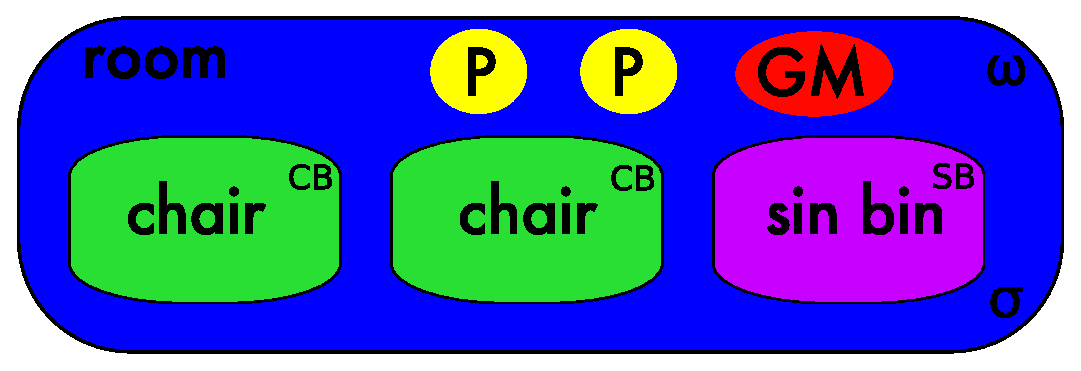
\includegraphics[scale=0.5]{gameenv}
  \caption{The Musical Chairs Environment}
  \label{fig:gameenv}
\end{figure}

The locality structure is represented graphically by Fig. \ref{fig:gameenv}
and in the calculus by the equation shown below.

\begin{equation}
\loc{room}{\nloc{chair}{\nil}{CB} \pc \nloc{chair}{\nil}{CB}
\pc \dots}{\Omega}{\sigma}
\end{equation}

\noindent where $\nloc{m}{E}{F}$ is abbrieviated from
$\loc{m}{E}{F}{\{\}}$.  The players themselves are represented by
\emph{processes}.  This allows them both to interact and to move between
localities.  A gamesmaster process is also introduced.  This doesn't
play an active role in the game itself, but is instead responsible for
performing the administrative duties of removing chairs from the game
and controlling player movement.  The process definitions are summarised
in Table \ref{tab:musicalchairs}, and make use of the derived syntax for
a clock prefix, $\sigma.P$, shown in \ref{clockcontrol}.

\begin{table}[h]
  \caption{Summary of Processes and Derived Syntax for Musical Chairs}
  \label{tab:musicalchairs}
  \shrule
  \begin{align}
   \omega &
     \eqdef 
     \mu X.(\overline{in}.X + \overline{out}.X + \overline{open}.X) \label{o}\\
   \sigma.P &
     \eqdef 
     \stimeout{\nil}{\sigma}{P} \label{clockpref} \\
   CB &
    \eqdef 
    \mu X.(\overline{in}.\overline{out}.X + \overline{open}) \label{chairb} \\
   SB &
    \eqdef 
    \mu X.\overline{in}.X \label{sinb} \\
   GM2 &
    \eqdef 
    \sigma.GM3 \label{gmstage2} \\
    GM3 &
    \eqdef 
    open\ chair.GM5 \label{gmstage3} \\
   GM4 &
   \eqdef
   \sigma.GM4 \label{gmstage4} \\
   GM5 &
    \eqdef  
    \mu X.(\stimeout{in\ chair\ sit.X}{\sigma}{GM6}) \label{gmstage5} \\
   GM6 &
    \eqdef 
    \mu X.(\stimeout{in\ sinbin\ leave.X}{\sigma}{GM2}) \label{gmstage6}\\
    Player &
    \eqdef 
    \stimeout{sit.PInChair}{\sigma}{Loser} \label{player}\\
   PInChair &
    \eqdef 
    \sigma.\sigma.PLeaveChair \label{pinchair} \\
   PLeaveChair &
   \eqdef
   out\ chair\ stand.0|stand.\sigma.\sigma.Player \label{pleavechair} \\
   Loser &
    \eqdef 
    leave.0 \label{loser} 
  \end{align}
  \shrule
\end{table}

The presence of music is signified by the ticks of a clock, $\sigma$.  A
tick from $\sigma$ is also used to represent the implicit
acknowledgement that everyone who can obtain a chair has done so, and
that the remaining player left in the room has lost.  With regard to the
bouncers of the localities, the room locality is not prone to either
destruction or the entry or exit of other localities, having a bouncer
simply equal to $\Omega$.  This retains the encapsulation of the model
as a single room locality, and prevents other processes or localities
from interfering with its behaviour.

The definition of appropriate bouncers is essential for the chairs
(\ref{chairb}) and the sin bin (\ref{sinb}).  It is the chair bouncer
that enforces the implicit predicate that only one player may inhabit a
chair at any one time, while the sin bin bouncer prevents players
leaving the sin bin once they have entered.

To model stage one of the game, $n$ player processes and $n$ chair
locations are placed in the room.  The advantage of using TNT for this
model is that the actual number of players or chairs is irrelevant.
They only have to be equal at the start to accurately model the game.
The calculus allows the creation of a compositional semantics, as
discussed in chapter \ref{introduction}, which work with any $n$.

For the purposes of demonstration, $n$ is assumed to be two to give the
following starting state:

\begin{equation}
  \loc{room}{\nloc{chair}{\nil}{CB} \pc \nloc{chair}{\nil}{CB} \pc 
   \sigma.\sigma.Player \pc \sigma.\sigma.Player \pc GM2}{\Omega}{\sigma}.
\end{equation}

\noindent The room and chairs appear as shown earlier.  The
processes of the form $\sigma.\sigma.Player$ simply wait until two clock
cycles have passed, the end of each being signalled by a tick from
$\sigma$.  The intermittent period between the ticks (the second clock
cycle) represents the playing of the music.  

Stage two, where the music is started, is thus represented simply by the
first tick of $\sigma$,

\begin{equation}
\begin{aligned}
  & \loc{room}{\nloc{chair}{\nil}{CB} \pc \nloc{chair}{\nil}{CB} \pc 
   \sigma.\sigma.Player \pc \sigma.\sigma.Player \pc
   GM2}{\Omega}{\sigma} \\
 \lderives{\sigma}\ & \loc{room}{\nloc{chair}{\nil}{CB} \pc \nloc{chair}{\nil}{CB} \pc 
   \sigma.Player \pc \sigma.Player \pc
   GM3}{\Omega}{\sigma}
\end{aligned}
\end{equation}

\noindent which the gamesmaster ($GM2$ (\ref{gmstage2})) also waits for,
before evolving in to $GM3$ (\ref{gmstage3}).  The second cycle, prior
to the music stopping, is used to remove a chair from the game.  Maximal
progress, as explained in section \ref{introduction}, ensures that this
occurs before the next clock tick, as the removal emits a silent action.
The transition from stage three to stage four is thus as follows:

\begin{equation}
\begin{aligned}
& \loc{room}{\nloc{chair}{\nil}{CB} \pc \nloc{chair}{\nil}{CB} \pc 
   \sigma.Player \pc \sigma.Player \pc
   GM3}{\Omega}{\sigma} \\
 \lderives{\tau}\ & \loc{room}{\nil \pc \nloc{chair}{\nil}{CB} \pc 
   \sigma.Player \pc \sigma.Player \pc
   GM4}{\Omega}{\sigma}
\end{aligned}
\end{equation}

\noindent with one of the two chairs being chosen non-deterministically.
The second tick then occurs, leading in to stage five and the most
interesting part of the model.

\begin{equation}
\begin{aligned}
& \loc{room}{\nil \pc \nloc{chair}{\nil}{CB} \pc 
   \sigma.Player \pc \sigma.Player \pc
   GM4}{\Omega}{\sigma} \\
\lderives{\sigma}\ & \loc{room}{\nil \pc \nloc{chair}{\nil}{CB} \pc 
   Player \pc Player \pc
   GM5}{\Omega}{\sigma} \\
\end{aligned}
\end{equation}

The aim of stage five is to get as many player processes as possible
inside chair localities.  This is handled by again relying on maximal
progress to essentially perform a form of broadcast that centres on
mobile actions, as briefly mentioned in \ref{procmob}.  Rather than
sending a signal to a number of recipients, a request to move into a
chair (see (\ref{gmstage5}) and (\ref{player})) is delivered instead.

If a chair is available, then a player process will enter it (the actual
chair and player chosen is non-deterministic).  This will cause an
internal action to occur, which takes precedence over the clock tick.
Thus, when the clock eventually does tick, it is clear that no more
players can enter chairs. Using clocks in this manner makes the system
\emph{compositional}; in contrast to other models, players and chairs
can be added without requiring changes to the process definitions.  In
this running example, there are two players, but only one chair, which
results in a single $\tau$ transition:

\begin{equation}
\begin{aligned}
& \loc{room}{\nil \pc \nloc{chair}{\nil}{CB} \pc 
   Player \pc Player \pc
   GM5}{\Omega}{\sigma} \\
\lderives{\tau}\ & \loc{room}{\nil \pc \nloc{chair}{\nil \pc PInChair}{\overline{out}.CB} \pc 
   Player \pc
   GM5}{\Omega}{\sigma} \\
\end{aligned}
\end{equation}

\noindent that causes one of the $Player$ processes to move in to a
chair, and become a $PInChair$ process.  This is followed by the
$\sigma$ transition, which marks the move to stage six.

\begin{equation}
\begin{aligned}
&  \loc{room}{\nil \pc \nloc{chair}{\nil \pc PInChair}{\overline{out}.CB} \pc 
   Player \pc
   GM5}{\Omega}{\sigma} \\
\lderives{\sigma}\ & \loc{room}{\nil \pc \nloc{chair}{\nil \pc \sigma.PLeaveChair}{\overline{out}.CB} \pc 
   Loser \pc
   GM6}{\Omega}{\sigma} \\
\end{aligned}
\end{equation}

Both stage six and seven proceed in a similar way.  Stage six sees
essentially the same broadcasting behaviour applied to the losing
players (see (\ref{gmstage6}) and (\ref{loser})).  The difference is
that stage six demonstrates something which wouldn't be possible without
mobility: the broadcast is limited to those player processes which
remain in the room.  As communication between processes in different
localities is disallowed in TNT, an implicit scoping of the broadcast
occurs.  In the example, stage six again sees just one $\tau$
transition:

\begin{equation}
\begin{aligned}
&  \loc{room}{\nil \pc \nloc{chair}{\nil \pc \sigma.PLeaveChair}{\overline{out}.CB} \pc 
   Loser \pc
   GM6}{\Omega}{\sigma} \\
\lderives{\tau}\ & \loc{room}{\nil \pc \nloc{chair}{\nil \pc \sigma.PLeaveChair}{\overline{out}.CB} \pc
   GM6}{\Omega}{\sigma} \\
\end{aligned}
\end{equation}

\noindent which results in the remaining $Player$ (now a $Loser$
process) moving to the sin bin.  Due to space constraints, the sin bin
locality is not shown in the above derivations.  It may be factored in
to the above as follows:

\begin{equation}
\begin{aligned}
& \nloc{sinbin}{\nil}{SB} \pc Loser \pc GM6 \\
\lderives{\tau} & \nloc{sinbin}{\nil \pc \nil}{SB} \pc GM6
\end{aligned}
\end{equation}

\noindent where the $Loser$ process evolves to become a simple $\nil$
process.  The broadcast is again terminated by a tick from $\sigma$,

\begin{equation}
\begin{aligned}
&  \loc{room}{\nil \pc \nloc{chair}{\nil \pc \sigma.PLeaveChair}{\overline{out}.CB} \pc
   GM6}{\Omega}{\sigma} \\
\lderives{\sigma}\ & \loc{room}{\nil \pc \nloc{chair}{\nil \pc PLeaveChair}{\overline{out}.CB} \pc
   GM2}{\Omega}{\sigma} 
\end{aligned}
\end{equation}

\noindent which, in this case, also signifies the music starting up again.  The
remaining players leave their chairs:

\begin{equation}
\begin{aligned}
& \loc{room}{\nil \pc \nloc{chair}{\nil \pc PLeaveChair}{\overline{out}.CB} \pc
   GM2}{\Omega}{\sigma}   \\
\lderives{\tau}\ & \loc{room}{\nil \pc \nloc{chair}{\nil \pc \nil}{CB} \pc
   GM2 \pc \sigma.\sigma.Player}{\Omega}{\sigma} 
\end{aligned}
\end{equation}

\noindent and the system essentially returns to the beginning, with $n -
1$ chairs and $n - 1$ players.

\section{The Type System}
\label{typesys}

This final section focuses on the beginnings of a type system for the
calculus.  The concepts behind this are based on the type systems
presented for the ambient calculus (see \ref{ambienttypes}) and
specifically the notion of groups presented in \cite{ambienttypes} and
\cite{m3}.  The current focus is on further restricting mobility, this
time limiting which process may move rather than how many, as is implied
by the bouncers of \ref{bouncers}.  The type system also provides the
distinction between normal process primitives and the primitives used by
bouncers, which is implicit in the examples above.

Each process and locality is a member of a group, which determines the
use of the mobility primitives.  Each group has a type\footnote{Or, as
groups are types themselves, it essentially has a type of a type or a
\emph{kind}}, $(\mathscr{C}, \mathscr{S}, \mathscr{O})$, with each
element being a set of groups.  Entities in groups that are members of
$\mathscr{C}$ are allowed to cross or pass through localities in the
given group.  For example, if $g_1$ has type $G_1$, where
$\mathscr{C}(G_1)$ is ${g_2}$, then localities or processes in group
$g_2$ may cross through localities in $g_1$.  In the same way,
$\mathscr{S}$ is the set of groups that may stay in a locality of that
group.  This is implicity a subset of $\mathscr{C}$ as, if a locality
can be stayed in, it must be crossable too.  Finally, $\mathscr{O}$
controls the members of which groups may destroy the locality via the
$open$ primitive.

Table \ref{tab:basictypes} presents the basic rules and the rudimentary
types used for the basic parts of the syntax, such as $\nil$.  As is
standard in the literature, the types are defined with respect to a type
environment, $\Gamma$.  On this note, the rule $Env$ simply states that
if $\xi$ of type $T$ is a member of $\Gamma$, then a typing derivation
$\vdash \xi : T$ may be made in the context of $\Gamma$.  This forms the
basis of all later rules.

\begin{table}
  \caption{Types: Basics}
  \label{tab:basictypes}
  \shrule
 \begin{center}
 \begin{tabular}{rc}
     \Rule{Env}
     {\xi : T \in \Gamma}
     {\Gamma \vdash \xi : T}
     {}
  &
  \Rule{Nil}
     {-}
     {\Gamma \vdash \nil : Proc(g)}
     {}
  \\[3ex]
     \Rule{BNil}
     {-}
     {\Gamma \vdash \Omega : BProc}
     {}
     &
     \Rule{Stop}
     {-}
     {\Gamma \vdash \Delta : Proc(g)}
     {}
     \\[3ex]
     \Rule{Stall}
     {\Gamma \vdash \sigma : Clock}
     {\Gamma \vdash \Delta_\sigma : Proc(g)}
     {}
     &
     \Rule{Act}
     {\Gamma \vdash \alpha : Act,
     \Gamma \vdash P : Proc (g)}
     {\Gamma \vdash \alpha . P : Proc(g)}
     {}
  \\[3ex]
     \Rule{Rec}
     {\Gamma \vdash P : Proc(g)}
     {\Gamma \vdash \mu X.P : Proc(g)}
     {}
     &
     \Rule{Res}
     {\Gamma \vdash a : Act,
     \Gamma \vdash P : Proc (g)}
     {\Gamma \vdash P \setminus a : Proc(g)}
     {}
 \end{tabular}
  \end{center}
  \shrule
\end{table}

The remaining rules in Table \ref{tab:basictypes} provide types for the
processes.  Via $Nil$ and $Stop$, both $\nil$ and $\Delta$ are given a
type of $Proc(g)$, where $g$ is a group.  There are no preconditions for
these derivations.  Likewise, $\Omega$ can be typed as a $BProc$, a
bouncer process, thus distinguishing it from the normal processes, such
as $\nil$.

The other rules are also pretty simple.  $Stall$ simply says that
$Delta_{\sigma}$ may be typed as a process of group $g$ if $\sigma$ is a
clock.  $Act$ states that $\alpha.P$ is a process in $g$ if $\alpha$ is
an action and $P$ is also typeable as a process in the same group.  In
the same vein, $Rec$ and $Res$ type recursive and restricted processes
respectively, if the constituent process, $P$, is already typeable as a
process.  In the case of $Res$, $a$ must also be an action if the
process is to be successfully typed.

In Table \ref{tab:operatortypes}, types are given to the composition of
processes using the binary operators for summation, parallel composition
and timeout.  All four are pretty much identical, providing a type for
the process resulting from the combination of the operator with two
other processes, $P$ and $Q$.  As each of these processes may be typed
under a different type environment (represented by $\Gamma_1$ and
$Gamma_2$), the cumulative process is typed under the union of the two,
on the condition that the two are compatible ($\Gamma_1 \# \Gamma_2$).
Compatibility is possible if there is no overlap between the two
environments.  Such overlap occurs when both environments provide a
different type for the same entity.  

\begin{table}
  \caption{Types: Operators}
  \label{tab:operatortypes}
  \shrule
 \begin{center}
 \begin{tabular}{c}
     \Rule{Sum}
     {\Gamma_1 \vdash P : Proc(g),
      \Gamma_2 \vdash Q : Proc(g),
      \Gamma_1 \# \Gamma_2}
     {\Gamma_1 \cup \Gamma_2 \vdash P + Q : Proc(g)}
     {}
     \\[3ex]
     \Rule{Par}
     {\Gamma_1 \vdash P : Proc(g),
      \Gamma_2 \vdash Q : Proc(g),
      \Gamma_1 \# \Gamma_2}
     {\Gamma_1 \cup \Gamma_2 \vdash P \;|\; Q : Proc(g)}
     {}
     \\[3ex]
     \Rule{FTO}
     {\Gamma_1 \vdash P : Proc(g),
      \Gamma_2 \vdash Q : Proc(g),
      \Gamma_1 \# \Gamma_2,
      \Gamma_1 \cup \Gamma_2 \vdash \sigma : Clock}
     {\Gamma_1 \cup \Gamma_2 \vdash \timeout{P}{\sigma}{Q} : Proc(g)}
     {}
  \\[3ex]
  \Rule{STO}
  {\Gamma_1 \vdash P : Proc(g),
      \Gamma_2 \vdash Q : Proc(g),
      \Gamma_1 \# \Gamma_2,
      \Gamma_1 \cup \Gamma_2 \vdash \sigma : Clock}
     {\Gamma_1 \cup \Gamma_2 \vdash \stimeout{P}{\sigma}{Q} : Proc(g)}
     {}
     \\[3ex]
 \end{tabular}
  \end{center}
  \shrule
\end{table}

The only other issue worthy of note with respect to these rules is that
$FTO$ and $STO$ also require that $\sigma$ is typeable as a clock,
another restriction which simply makes explicit a number of issues
implied in the syntax.

The types in Tables \ref{tab:basictypes} and \ref{tab:operatortypes}
provide the basis for the mobility types presented in Table
\ref{tab:mobilitytypes}, which form the focus of the type system.  This
table is so far incomplete, as it lacks typing for process mobility and
the rule to link processes and localities.  The latter exists, but may
need further work.  These issues are discussed in \ref{futuretypes}.

\begin{table}
  \caption{Types: Mobility}
  \label{tab:mobilitytypes}
  \shrule
 \begin{center}
 \begin{tabular}{c}
     \Rule{Cap}
     {\Gamma \vdash \ambop : Proc(g_1) \rightarrow Proc(g_2),
     \Gamma \vdash P : Proc (g_1)}
     {\Gamma \vdash \ambop . P : Proc(g_2)}
     {}
     \\[3ex]
     \Rule{LocIn}
     {\Gamma \vdash g_2 : G_2,
      \Gamma \vdash m : Loc(g_1),
      g_1 \in \mathscr{C}(G_2)}
     {\Gamma \vdash \ambin{m} : Proc(g_2) \rightarrow Proc(g_2)}
     {}
     \\[3ex]
     \Rule{LocOut\ }
     {\Gamma \vdash g_1 : G_1, 
      \Gamma \vdash g_2 : G_2,
      \Gamma \vdash m : Loc(g_1),
      g_1 \in \mathscr{C}(G_2),
      \mathscr{S}(G_1) \subseteq \mathscr{S}(G_2)}
     {\Gamma \vdash \ambout{m} : Proc(g_2) \rightarrow Proc(g_2)}
     {}
     \\[3ex]
     \Rule{Open}
     {\Gamma \vdash g_1 : G_1,
      \Gamma \vdash g_2 : G_2,
      \Gamma \vdash m : Loc(g_1),
      g_1 \in \mathscr{O}(G_2),
      g_2 \in \mathscr{S}(G_1)}
     {\Gamma \vdash \ambopen{m} : Proc(g_2) \rightarrow Proc(g_2)}
     {}
 \end{tabular}
  \end{center}
  \shrule
\end{table}

Of the ones presented here, $LocIn$, $LocOut$ and $Open$ are fairly
similar, all relating to whether a particular location movement is
typeable, based on the groups of the localities and the processes within
them.  $Cap$ differs in that it provides the actual change in type that
occurs when the movement takes place.  Its behaviour is akin to function
composition.  

Within the type system, mobility primitives are given function types, to
represent the fact that they may cause a transition from one group to
another\footnote{This is not evident in the rules given, as the
processes move as part of the locality, and thus stay in the same
group.  Such changes occur in process movement, where the locality of a
process changes, and thus its group.}.  The rule itself simply states
that if $\ambop$ has a function type, transforming processes of the
group $g_1$ to a process in the group $g_2$, and $P$ is a process in
group $g_1$, then $\ambop.P$ is typed as the result of applying $\ambop$
to $P$, to give a process in group $g_2$.

The function types used for this are generated by rules like $LocIn$,
$LocOut$ and $Open$, which are specific to each mobility primitive.
$LocIn$ states that if $m$ is a locality of group $g_1$, then
$\ambin{m}$ is typeable as $Proc(g_2) \rightarrow Proc(g_2)$ if the
group $g_1$ is one of the members of the set of crossable localities
maintained by $G_2$, the type of the group, $g_2$, used by the process
emitting the capability.

The other two rules run along the same lines.  $LocOut$ is nearly the
same, except that the set of locality groups where members of $g_1$ can
stay must be a subset of the set in which members of $g_2$ can stay.
This is because the moving locality, in $g_1$, must be able to stay in
the locality in which $m$ (a member of $g_2$) is currently situated,
when it moves outside it.

Finally, the rule for $Open$ states that $g_1$, the group of the
locality being opened, must be a member of the set of groups that are
openable by members of $g_2$ and that $g_2$ must be a member of the set
of groups that can stay in localities of group $g_1$.  The latter
condition is necessary to ensure that the contents of the destroyed
locality are allowed to enter the parent locality.



\chapter{Future Work}


\addcontentsline{toc}{section}{Bibliography}
\bibliography{literature}
\bibliographystyle{acm}



\end{document}
